% Use the following line _only_ if you're still using LaTeX 2.09.
%\documentstyle[icml2015,epsf,natbib]{article}
% If you rely on Latex2e packages, like most moden people use this:
\documentclass{article}

% use Times
\usepackage{times}
% For figures
\usepackage{graphicx} % more modern
%\usepackage{epsfig} % less modern
%\usepackage{subfigure} 
\usepackage{float}

% For citations
\usepackage{natbib}

% For algorithms
\usepackage{algorithm}
\usepackage{algorithmic}

% As of 2011, we use the hyperref package to produce hyperlinks in the
% resulting PDF.  If this breaks your system, please commend out the
% following usepackage line and replace \usepackage{icml2015} with
% \usepackage[nohyperref]{icml2015} above.
\usepackage[hypertexnames=false]{hyperref}

% Packages hyperref and algorithmic misbehave sometimes.  We can fix
% this with the following command.
\newcommand{\theHalgorithm}{\arabic{algorithm}}

% Employ the following version of the ``usepackage'' statement for
% submitting the draft version of the paper for review.  This will set
% the note in the first column to ``Under review.  Do not distribute.''
%\usepackage{icml2015}

% Employ this version of the ``usepackage'' statement after the paper has
% been accepted, when creating the final version.  This will set the
% note in the first column to ``Proceedings of the...''
\usepackage[accepted]{icml2015}


\graphicspath{{figures/}}

% JBY Custom stuff
\usepackage{amsmath}
\usepackage{amssymb}
\usepackage{ownstyles}

\DeclareMathOperator*{\argmax}{arg\,max}
\newcommand{\x}{\mathbf{x}}
\newcommand{\xs}{\mathbf{x^*}}
\newcommand{\xn}{\mathbf{x_0}}

\newcommand{\layer}[1]{\ensuremath{\mathsf{#1}\xspace}}
\newcommand{\unit}[2]{\ensuremath{\mathsf{#1_{#2}}\xspace}}
%\newcommand{\baseA}{\net{baseA}}
%\newcommand{\baseB}{\net{baseB}}
%%\newcommand{\dA}{$A$\xspace}
%%\newcommand{\dB}{$B$\xspace}
%\newcommand{\dA}{\net{A}\xspace}
%\newcommand{\dB}{\net{B}\xspace}
%%\newcommand{\capemph}[1]{\textbf{#1}}
%\newcommand{\capemph}[1]{\emph{#1}}


% % Commenting highlights
\newif\ifcomments

%Uncomment one of the two lines below to turn todos on/off
%\commentsfalse
\commentstrue

\ifcomments
\newcommand{\comments}[1]{#1}
\else
\newcommand{\comments}[1]{}
\fi
% % Commenting highlights


%\newcommand{\titl}{Visualizing Deep Neural Networks through Interaction and Optimization}

\newcommand{\titl}{Understanding Neural Networks Through Deep Visualization}
\newcommand{\suptitl}{Supplementary Information for:\\\titl}
\newcommand{\suptitlrunning}{Supplementary Information for: \titl}



% The \icmltitle you define below is probably too long as a header.
% Therefore, a short form for the running title is supplied here:
\icmltitlerunning{\titl}

\pagestyle{plain}
\setlength{\footskip}{20pt}    % Move page numbers down a little

\begin{document} 

\twocolumn[
  \icmltitle{\titl}

% It is OKAY to include author information, even for blind
% submissions: the style file will automatically remove it for you
% unless you've provided the [accepted] option to the icml2015
% package.
\icmlauthor{Jason Yosinski}{yosinski@cs.cornell.edu}
\icmladdress{Cornell University}
\icmlauthor{Jeff Clune}{jeffclune@uwyo.edu}
%\icmladdress{University of Wyoming}
\icmlauthor{Anh Nguyen}{anguyen8@uwyo.edu}
\icmladdress{University of Wyoming}
\icmlauthor{Thomas Fuchs}{fuchs@caltech.edu}
\icmladdress{Jet Propulsion Laboratory, California Institute of Technology}
\icmlauthor{Hod Lipson}{hod.lipson@cornell.edu}
\icmladdress{Cornell University}

% You may provide any keywords that you 
% find helpful for describing your paper; these are used to populate 
% the "keywords" metadata in the PDF but will not be shown in the document
\icmlkeywords{convolutional neural networks, neural networks, visualization}

\vskip 0.3in
]

\begin{abstract}
Recent years have produced great advances in training
  large, deep neural networks (DNNs), including notable successes in training
  convolutional neural networks (convnets) to recognize natural images. However,
  our understanding of how these models work, especially what
  computations they perform at intermediate layers, has lagged
  behind. Progress in the field will be further accelerated by the development of
  better tools for visualizing and interpreting  neural nets.
  We introduce two such tools here. The first
  is a tool that visualizes the activations produced on each layer
  of a trained convnet as it processes an image or video (e.g. a live webcam stream). We have found that looking at live activations that change in response
  to user input helps build valuable intuitions about how convnets work. The second tool enables visualizing features at each
  layer of a DNN via regularized optimization in image space. Because previous versions of this idea produced less recognizable images, here
  we introduce several new regularization methods that combine to produce qualitatively clearer, more interpretable visualizations. Both tools are open source and work on a pre-trained convnet with minimal setup.
\end{abstract}



\section{Introduction}
\label{introduction}


The last several years have produced tremendous progress in training powerful, deep neural network models that are approaching and even surpassing human abilities on a variety of challenging machine learning tasks \cite{taigman-2014-CVPR-deepface:-closing-the-gap-to-human-level,schroff-2015-arXiv-facenet:-a-unified-embedding,hannun-2014-arXiv-deep-speech:-scaling}. A flagship example is training deep, convolutional neural networks (CNNs) with supervised learning to classify natural images \cite{krizhevsky2012imagenet-classification-with-deep}. That area has benefitted from the combined effects of faster computing (e.g. GPUs), better training techniques (e.g. dropout \cite{hinton2012improving-neural-networks-by-preventing}), better activation units (e.g. rectified linear units \cite{glorot-2011-AISTATS-deep-sparse-rectifier}), and larger labeled datasets  \cite{deng2009imagenet:-a-large-scale-hierarchical,lin-2014-arXiv-microsoft-coco-common}. 
%This paper focuses on one such convolutional model, colloquially dubbed ``AlexNet'', an eight layer convnet \cite{krizhevsky2012imagenet-classification-with-deep} trained using Caffe \cite{jia2014caffe:-convolutional-architecture} on the Imagenet Large Scale Visual Recognition Challenge (ILSVRC) 2012 dataset \cite{deng2009imagenet:-a-large-scale-hierarchical}.

%This recent progress toward better models has been driven in part by an influx of research interest, which in our estimation, has been driven by the combined effects of the easy availability of computation via GPUs, data, as well as increasingly mature software packages --- like Theano \cite{bergstra2010theano:-a-cpu-and-gpu-math-expression} and Pylearn2 \cite{goodfellow2013pylearn2:-a-machine-learning-research}, Caffe \cite{jia2014caffe:-convolutional-architecture}, and Torch \cite{collobert-2011-torch7:-a-matlab-like-environment} --- that allow easy experimentation with shallower learning curves.
%%To crystalize the point, it
%It is now possible for a new entrant to the field, say, a student in his or her first machine learning class, to download one of these software packages and train a model that attains or nearly attains state of the art in only a few lines of configuration or code. This ease of entry has increased the amount of research being done and has led to faster progress and more papers.

% CASUAL: it's now possible to train model with 8000099 parameters using 3 commands and standard software. But the output is a scalar.
% How much of our work centers around shuffling data in one format or another, staring at slowly decreasing error rates? When we finally get an error rate even lower: yay! But this is such a low-dimensional view of the underlying phenomena. We need higher-bandwidth tools as well.

%However, our understanding of how these large neural models operate has lagged behind. The computation performed by a trained neural network to be decomposed into two parts. First, we may examine the \emph{network architecture} as a skeleton of what could be. That is, we may try to understand the wide space of possible functions that could be expressed by some particular combination of dot products, pooling, nonlinearities, and so on. Second, we may seek to understand the particular function specified by the \emph{actual, learned network weights}. Having the former without the latter results in only a loose understanding, because the space of possible functions is vast. But the latter type of understanding is inherently difficult, because it entails making some sense of the values taken by a very large number of parameters, 60 million in the network used for this study.
% 60965224 parameters in our CaffeNet model

While there has thus been considerable improvements in our knowledge of how to create high-performing architectures and learning algorithms, our understanding of how these large neural models operate has lagged behind. Neural networks have long been known as ``black boxes'' because it is difficult to understand exactly how any particular, trained neural network functions due to the large number of interacting, non-linear parts. Large modern neural networks are even harder to study because of their size; for example, understanding the widely-used AlexNet DNN involves making sense of the values taken by the 60 million trained network parameters. Understanding what is learned is interesting in its own right, but it is also one key way of further improving models: the intuitions provided by understanding the current generation of models should suggest ways to make them better. For example, the deconvolutional technique for visualizing the features learned by the hidden units of DNNs suggested an architectural change of smaller convolutional filters that led to state of the art performance on the ImageNet benchmark in 2013~\cite{zeiler2013visualizing-and-understanding-convolutional}.

We also note that tools that enable understanding will especially benefit the vast numbers of newcomers to deep learning, who would like to take advantage of off-the-shelf software packages --- like Theano \cite{bergstra2010theano:-a-cpu-and-gpu-math-expression}, Pylearn2 \cite{goodfellow2013pylearn2:-a-machine-learning-research}, Caffe \cite{jia2014caffe:-convolutional-architecture}, and Torch \cite{collobert-2011-torch7:-a-matlab-like-environment} --- in new domains, but who may not have any intuition for why their models work (or do not). Experts can also benefit as they iterate ideas for new models or when they are searching for good hyperparameters. We thus believe that both experts and newcomers will benefit from tools that provide intuitions about the inner workings of DNNs.  This paper provides two such tools, both of which are open source so that scientists and practitioners can integrate them with their own DNNs to better understand them. 

The first tool is software that interactively plots the activations produced on each layer of a trained DNN for user-provided images or video. Static images afford a slow, detailed investigation of a particular input, whereas video input highlights the DNNs changing responses to dynamic input.  At present, the videos are processed live from a user's computer camera, which is especially helpful because users can move different items around the field of view, occlude and combine them, and perform other manipulations to actively learn how different features in the network respond.

\begin{figure*}[!th]
%\vskip 0.2in
\begin{center}
  \centerline{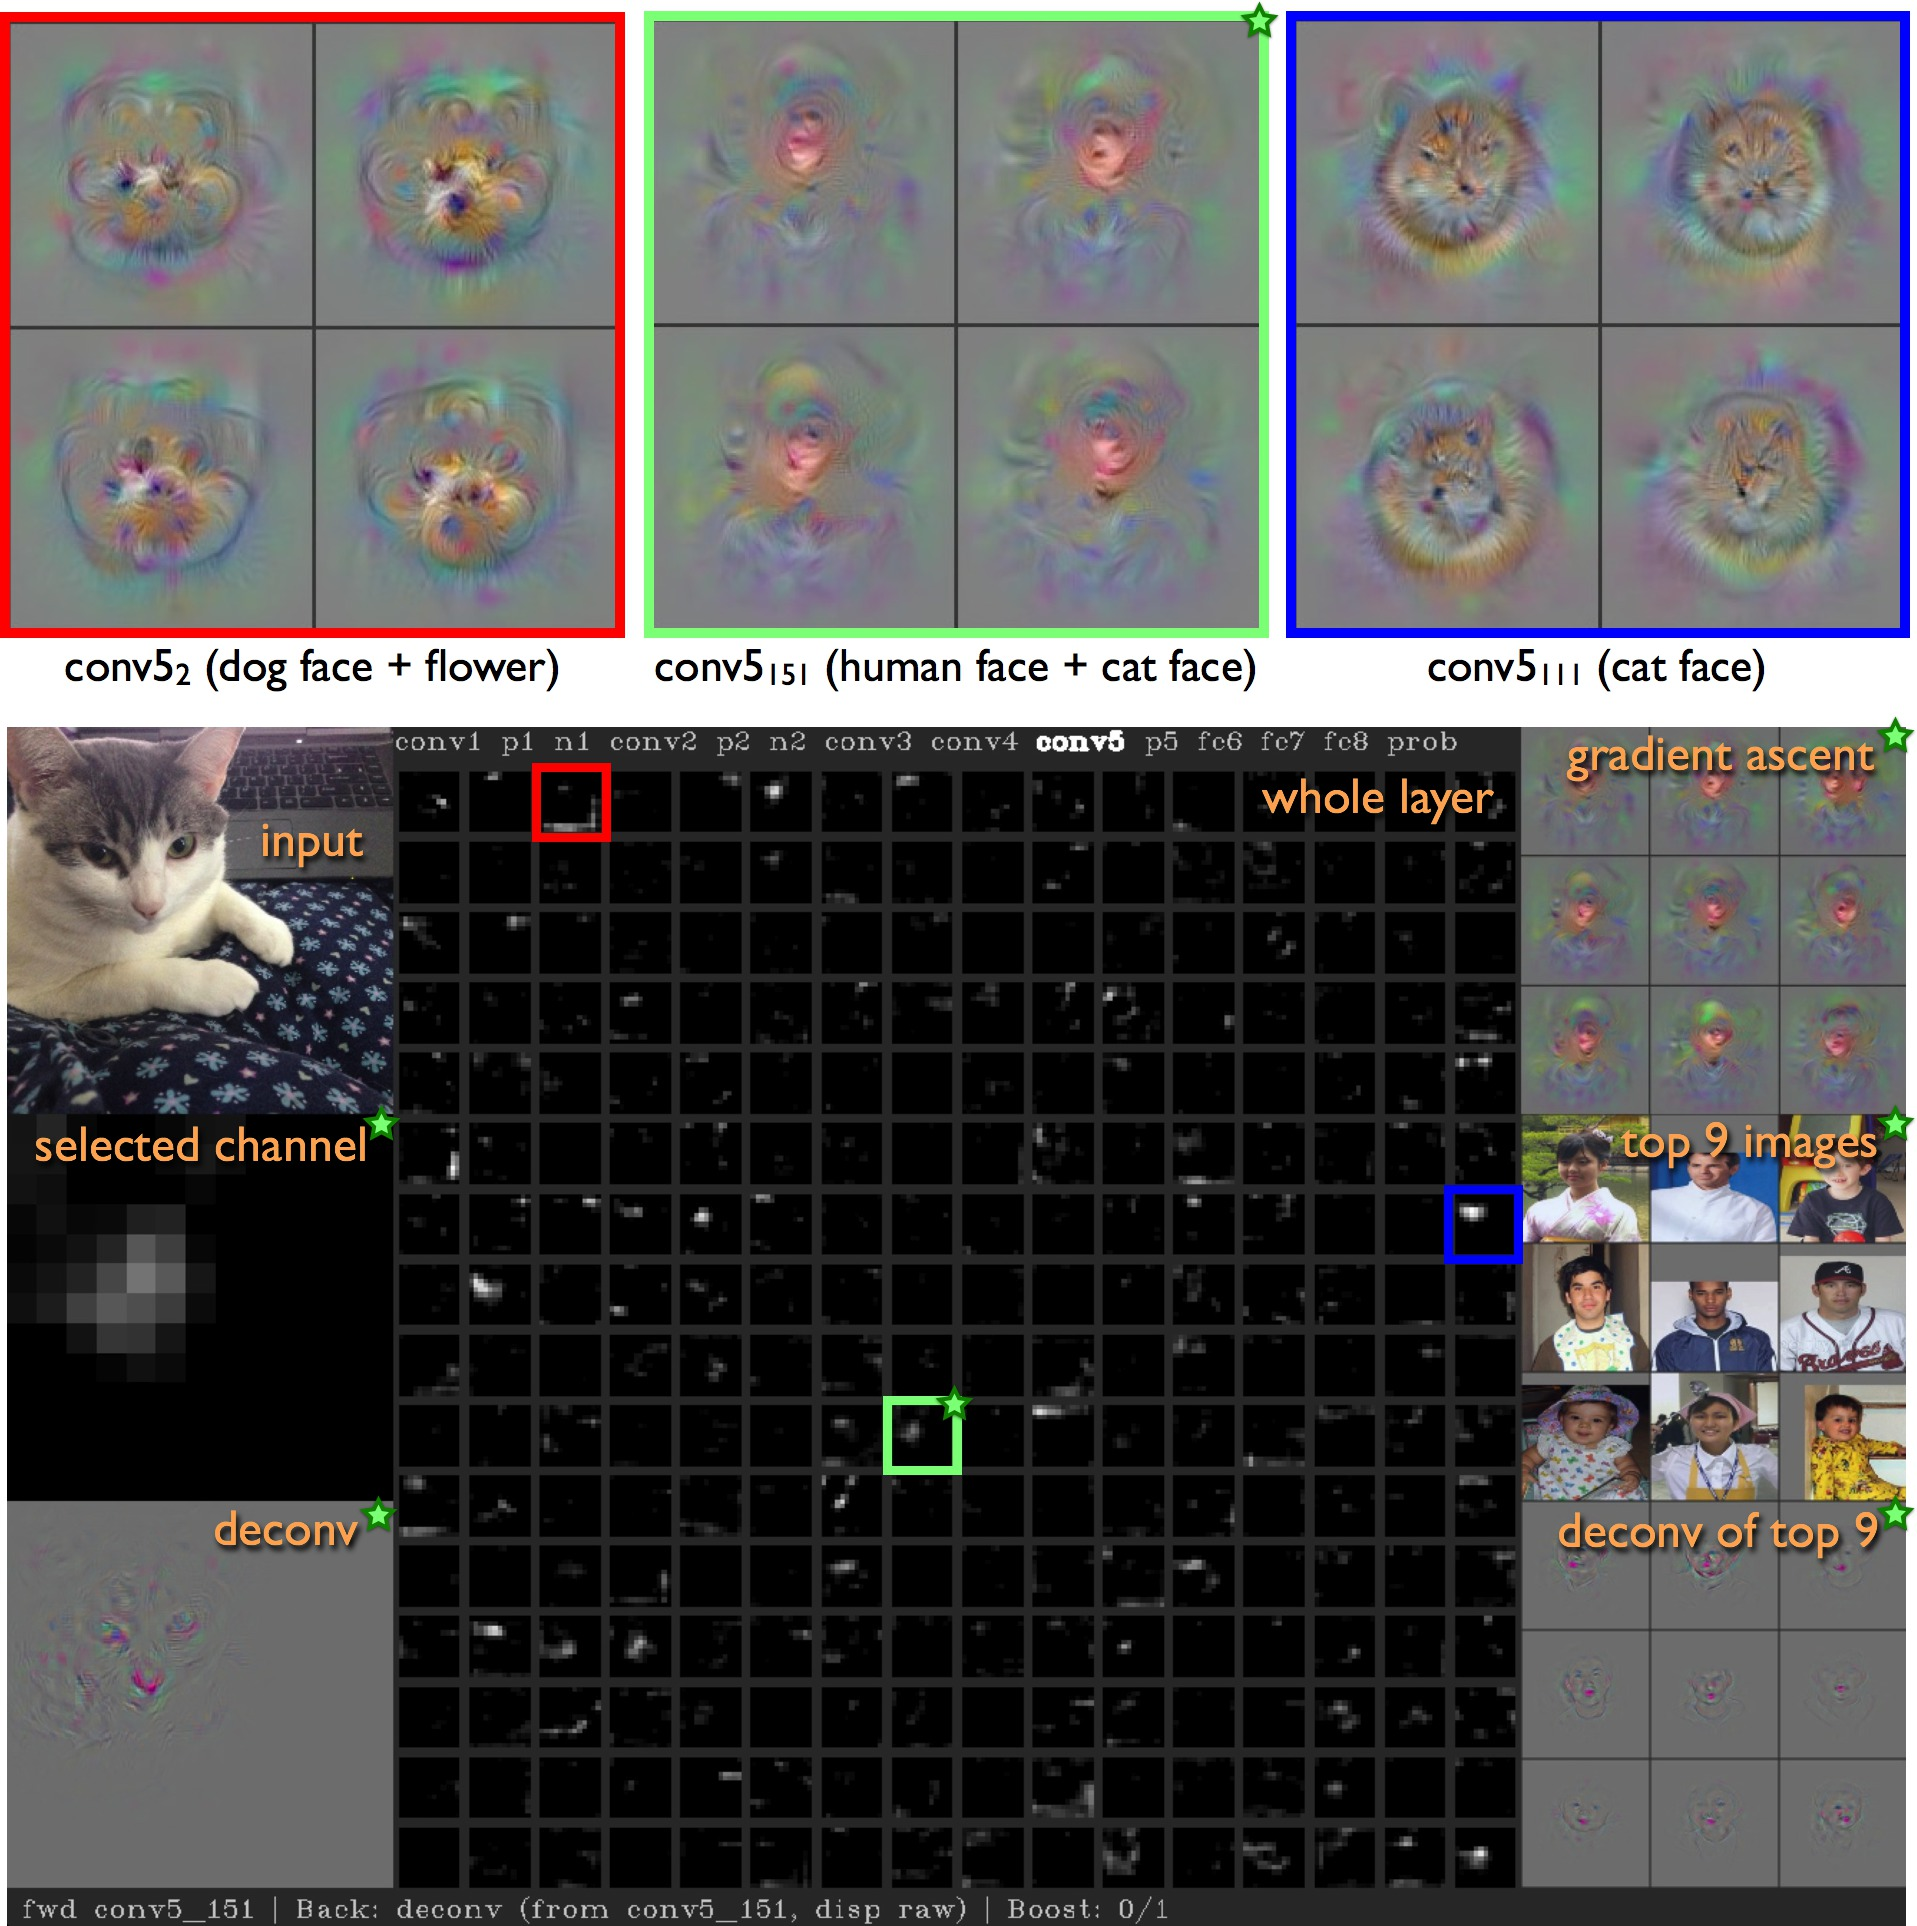
\includegraphics[width=1\linewidth]{demo_layers/demo_layers_2.jpg}}
  \vskip -.1in
\caption{The \textbf{bottom} shows a screenshot from the interactive visualization software. The webcam \emph{input} is shown, along with the \emph{whole layer} of \layer{conv5} activations. The \emph{selected channel} pane shows an enlarged version of the 13x13 \unit{conv5}{151} channel activations. Below it, the \emph{deconv} starting at the selected channel is shown. On the right, three selections of nine images are shown: synthetic images produced using the regularized \emph{gradient ascent} methods described in \secref{optimization}, the \emph{top 9 image} patches from the training set
  (the images from the training set that caused the highest activations for the selected channel),
  and the \emph{deconv of the those top 9} images. All areas highlighted with a green star relate to the particular selected channel, here \unit{conv5}{151}; when the selection changes, these panels update.
  % The webcam input is shown along with several selected layers. \layer{conv1} shows the 96 first layer filters learned. Due to the group structure imposed while training, a natural structure emerges where the first 48 filters (here: first 48 in row-major order) learn mostly grayscale edge filters and the second 48 learn mostly color blob detectors. Upon closer inspection, we can see that \unit{conv1}{43} and \unit{conv1}{44} detect low frequency left-right edges in alternate orientations. By \layer{conv5} the units are computing more abstract features that are invariant to many factors.
The \textbf{top} depicts enlarged numerical optimization results for this and other channels. \unit{conv5}{2} is a channel that responds most strongly to dog faces (as evidenced by the top nine images, which are not shown due to space constraints), but it also responds to flowers on the blanket on the bottom and half way up the right side of the image (as seen in the inset red highlight). This response to flowers can be partially seen in the optimized images but would be missed in an analysis focusing only on the top nine images and their deconv versions, which contain no flowers.
  %\todo{this argument is not very convincing without adding that figure}
\unit{conv5}{151} detects different types of faces. The top nine images are all of human faces, but here we see it responds also to the cat's face (and in \figref{demo_face} a lion's face). Finally, \unit{conv5}{111} activates strongly for the cat's face, the optimized images show catlike fur and ears, and the top nine images (not shown here) are also all of cats. For this image, the \layer{softmax} output layer top two predictions are ``Egyptian Cat'' and ``Computer Keyboard.'' All figures in this paper are best viewed digitally, in color, significantly zoomed in.
%\todo{Now, or for the CRC, can we change channel to neuron throughout (including in the figure)? More interesting to a broader community of people (neuroscientists, general audience, etc.)}
}
\figlabel{demo_layers}
\end{center}
\vskip -0.2in
\end{figure*}
% Here the top 5 contains three breeds of cat, computer keyboard, and computer mouse. Inset: The framework also allows visualizing activations arising from images in a directory. Here we show a gorilla picture from Flickr\footnote{Flickr user harlequeen, photo 7913344990} and it's correct classification as "Gorilla".}


%We originally conceived this as a quickly hacked together combination of OpenCV and Caffe in Python, but after playing with it for a while, it so quickly led to new intuition (see \secref{demo}) that we have packaged it in an easily installable way and made it available on Github (\url{http://yosinski.com/deepvis}) for researchers to apply to the own network models (or by using a pre-trained model we provide).

% in the field's understanding about how the models work, both on a deep theoretical level and on a simpler intuitive level. It is this second intuitive level of understanding that this paper

The second tool we introduce enables better visualization of the learned features computed by individual neurons at every layer of a DNN. Seeing what features have been learned is important both to understand how current DNNs work and to fuel intuitions for how to improve them. 

Attempting to understand what computations are performed at each layer in DNNs is an increasingly popular direction of research. One approach is to study each layer as a group and investigate the type of computation performed by the set of neurons on a layer as a whole~\cite{yosinski-2014-NIPS-how-transferable-are-features-in-deep,mahendran-2014-arXiv-understanding-deep-image}. This approach is informative because the neurons in a layer interact with each other to pass information to higher layers, and thus each neuron's contribution to the entire function performed by the DNN depends on that neuron's context in the layer. 

Another approach is to try to interpret the function computed by each individual neuron. Past studies in this vein roughly divide into two different camps: \emph{dataset-centric} and \emph{network-centric}. The former requires both a trained DNN and running data through that network; the latter requires only the trained network itself. One dataset-centric approach is to display images from the training or test set that cause high or low activations for individual units. Another is the deconvolution method of Zeiler \& Fergus~\yrcite{zeiler2013visualizing-and-understanding-convolutional}, which highlights the portions of a particular image that are responsible for the firing of each neural unit.
%a process that can be informative for high-level units, but becomes less-so for lower-level units, where one does not know which small part of the larger image caused the neuron to fire. 
%the representational power of the set of units on a layer as a whole \cite{yosinski-2014-NIPS-how-transferable-are-features-in-deep,mahendran-2014-arXiv-understanding-deep-image} and others on the computations performed by specific units.
%Both perspectives may be useful. 
%features are computed by units of a convnet, both when all units are considered at once, 
%computation is being performed by units of a convnet, both when viewed collectively at a layer level or individually. When considered collectively each individual unit in a neural network
%Two of the main approaches toward understanding the function of specific units have been 

Network-centric approaches investigate a network directly without any data from a dataset. For example, Erhan et al.~\yrcite{erhan2009visualizing-higher-layer-features} synthesized images that cause high activations for particular units. Starting with some initial input $\x = \xn$, the activation $a_i(\x)$ caused at some unit $i$ by this input is computed, and then steps are taken in input space
% is the function that maps from input $\x$ to the activation of $unit_i$.
along the gradient $\partial a_i(\x) /\partial \x$ to synthesize inputs that cause higher and higher activations of unit $i$, eventually terminating at some $\xs$ which is deemed to be a preferred input stimulus for the unit in question. In the case where the input space is an image, $\xs$ can be displayed directly for interpretation. Others have followed suit, using the gradient to find images that cause higher activations \cite{simonyan2013deep-inside-convolutional,nguyen-2014-arXiv-deep-neural-networks} or lower activations \cite{szegedy2013intriguing-properties-of-neural} for output units.

These gradient-based approaches are attractive in their simplicity, but the optimization process tends to produce images that do not greatly resemble natural images. Instead, they are composed of a collection of ``hacks'' that happen to cause high (or low) activations: extreme pixel values, structured high frequency patterns, and copies of common motifs without global structure~\cite{simonyan2013deep-inside-convolutional,nguyen-2014-arXiv-deep-neural-networks,szegedy2013intriguing-properties-of-neural,goodfellow-2014-arXiv-explaining-and-harnessing-adversarial}. The fact that activations may be effected by such hacks is better understood thanks to several recent studies. Specifically, it has been shown that such hacks may be applied to correctly classified images to cause them to be misclassified even via imperceptibly small changes \cite{szegedy2013intriguing-properties-of-neural}, that such hacks can be found even without the gradient information to produce unrecognizable ``fooling examples'' \cite{nguyen-2014-arXiv-deep-neural-networks}, and that the abundance of non-natural looking images that cause extreme activations can be explained by the locally linear behavior of neural nets 
%with rectified linear units 
\cite{goodfellow-2014-arXiv-explaining-and-harnessing-adversarial}.


With such strong evidence that optimizing images to cause high activations produces unrecognizable images, is there any hope of using such methods to obtain useful visualizations? It turns out there is, if one is able to appropriately regularize the optimization. Simonyan et al.~\yrcite{simonyan2013deep-inside-convolutional} showed that slightly discernible images for the final layers of a convnet could be produced with $L_2$-regularization. Mahendran and Vedaldi \yrcite{mahendran-2014-arXiv-understanding-deep-image} also showed the importance of incorporating natural-image priors in the optimization process when producing images that mimic an entire-layer's firing pattern produced by a specific input image. We build on these works and contribute three additional forms of regularization that, when combined, produce more recognizable, optimization-based samples than previous methods. Because the optimization is stochastic, by starting at different random initial images, we can produce a set of optimized images whose variance provides information about the invariances learned by the unit.

To summarize, this paper makes the following two contributions:


\begin{enumerate}

\item We describe and release a software tool that provides a live, interactive visualization of every neuron in a trained convnet as it responds to a user-provided image or video. The tool displays forward activation values, preferred stimuli via gradient ascent, top images for each unit from the training set, deconv highlighting \cite{zeiler2013visualizing-and-understanding-convolutional} of top images, and backward diffs computed via backprop or deconv starting from arbitrary units. The combined effect of these complementary visualizations promotes a greater understanding of what a neuron computes than any single method on its own. We also describe a few insights we have gained from using this tool.
%The software is relatively straightforward, so the primary contribution is that we have made the code easy to download, install, and use without high startup costs
(\secref{demo}).

%\item We extend past efforts to visualize preferred activation patterns in input space for units on higher layers. This general approach has been popularized by CITE Erhan. However, recent work has called into question the usefulness of computing patterns that cause high activity for high level neurons, because such neurons may be activated no only by representative examplars from a natural image training set, but also via clever hacks inserting just the right high frequency noise calculated via the gradient (CITE Intriguing) or by generating "fooling images" via evolutionary algorithms (CITE Anh). However, here we show that by including certain types of regularization, one can inject a prior that excludes many common hacks, instead finding relatively interpretable images (SECTION vis).

\item We extend past efforts to visualize preferred activation patterns in input space by adding several new types of regularization, which produce what we believe are the most interpretable images for large convnets so far (\secref{optimization}).

\end{enumerate}

Both of our tools are released as open source and are available at
\url{http://yosinski.com/deepvis}. While the tools could be adapted to integrate with any DNN software framework, they work out of the box with 
the popular Caffe DNN software package \cite{jia2014caffe:-convolutional-architecture}.
Users may run visualizations with their own Caffe DNN or our pre-trained DNN, which comes with pre-computed images optimized to activate each neuron in this trained network. Our pre-trained network is nearly identical to the ``AlexNet'' architecture \cite{krizhevsky2012imagenet-classification-with-deep}, but with local reponse normalization layers after pooling layers following \citep{jia2014caffe:-convolutional-architecture}. It was trained with the Caffe framework on the ImageNet 2012 dataset \cite{deng2009imagenet:-a-large-scale-hierarchical}. 





\section{Visualizing Live Convnet Activations}
\seclabel{demo}

%The usual process of inference in a trained convnet entails feeding an image into the bottom data layer of a convnet and then computing activations from the bottom up in a forward pass. 
Our first visualization method is straightforward:  plotting the activation values for the neurons in each layer of a convnet in response to an image or video. In fully connected neural networks, the order of the units is irrelevant, so plots of these vectors are not spatially informative. However, in convolutional networks, filters are applied in a way that respects the underlying geometry of the input; in the case of 2D images, filters are applied in a 2D convolution over the two spatial dimensions of the image. This convolution produces activations on subsequent layers that are, for each channel, also arranged spatially.

\figref{demo_layers} shows examples of this type of plot for the \layer{conv5} layer.
%\figref{demo_layers} shows several layers of various sizes. 
%For example the data input has size $3\times227\times227$ (channels $\times$ pixels $\times$ pixels), so we can plot it as a color image. 
The \layer{conv5} layer has size 256$\times$13$\times$13, which we depict as 256 separate 13$\times$13 grayscale images. Each of the 256 small images contains activations in the same spatial $x$-$y$ spatial layout as the input data, and the 256 images are simply and arbitrarily tiled into a 16$\times$16 grid in row-major order.
%\footnote{The only structure present in the ordering of the 96 channels is a separation into two connectivity groups of 48 \cite{krizhevsky2012imagenet-classification-with-deep}, connectivity that caused this particular network to learn the set of edge filters in the first 48 and color blobs in the second 48.}
\figref{demo_face} shows a zoomed in view of one particular channel, \unit{conv5}{151}, that responds to human and animal faces. All layers can be viewed in the software tool, including pooling and normalization layers. Visualizing these layers provides intuitions about their effects and functions.




\begin{figure}[!h]
\vskip 0.2in
\begin{center}
  %\includegraphics[width=.5\linewidth]{demo_face/wendy_03.jpg}\includegraphics[width=.5\linewidth]{demo_face/face_wendy_03.png} \\
  %\vspace{.5ex}
  %\includegraphics[width=.5\linewidth]{demo_face/wendy_02.jpg}\includegraphics[width=.5\linewidth]{demo_face/face_wendy_02.png} \\
  %\vspace{.5ex}
  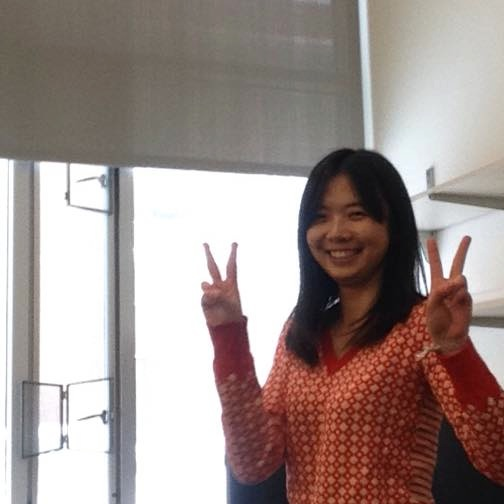
\includegraphics[width=.5\linewidth]{demo_face/wendy_06.jpg}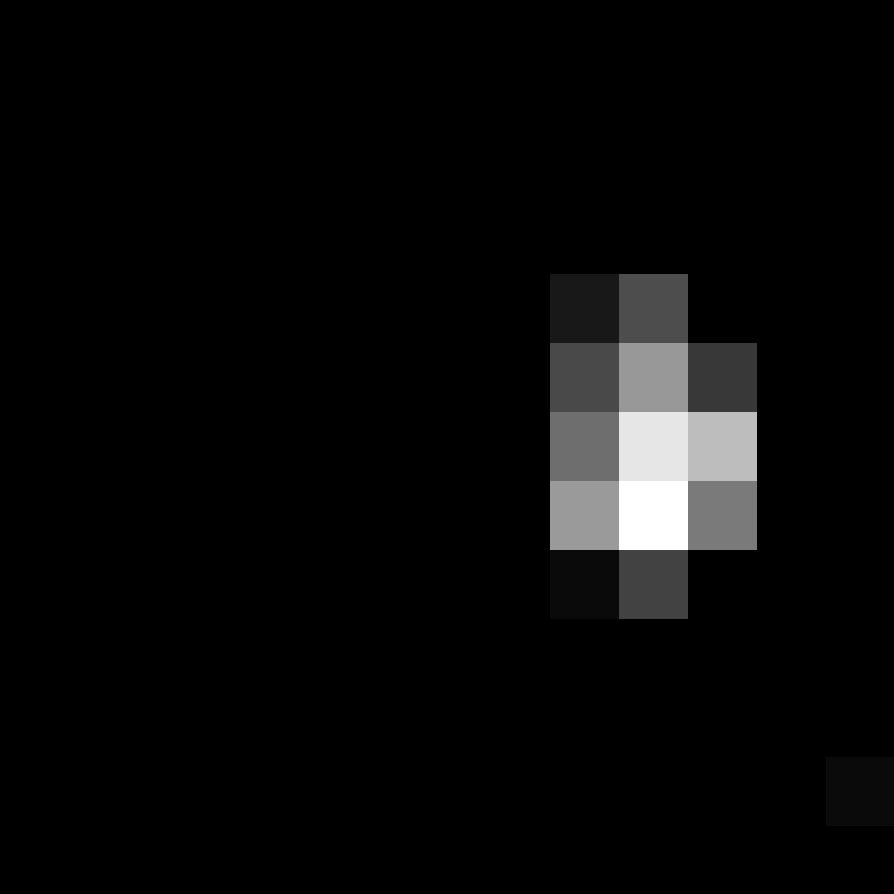
\includegraphics[width=.5\linewidth]{demo_face/face_wendy_06.png} \\
  \vspace{.5ex}
  %\includegraphics[width=.5\linewidth]{demo_face/sweater_woman.png}\includegraphics[width=.5\linewidth]{demo_face/face_sweater_woman.png} \\
  %\vspace{.5ex}
  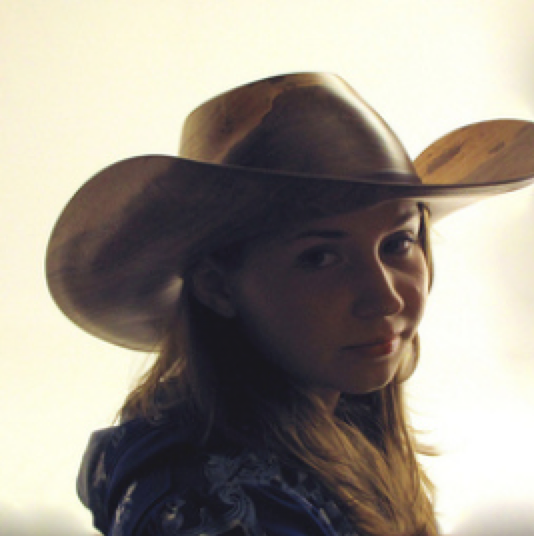
\includegraphics[width=.5\linewidth]{demo_face/hat_woman.png}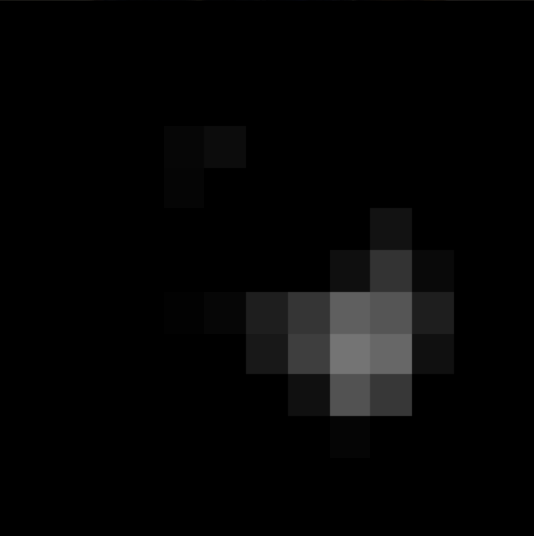
\includegraphics[width=.5\linewidth]{demo_face/face_hat_woman.png} \\
  \vspace{.5ex}
  %\includegraphics[width=.5\linewidth]{demo_face/jason.png}\includegraphics[width=.5\linewidth]{demo_face/face_jason.png} \\
  %\vspace{.5ex}
  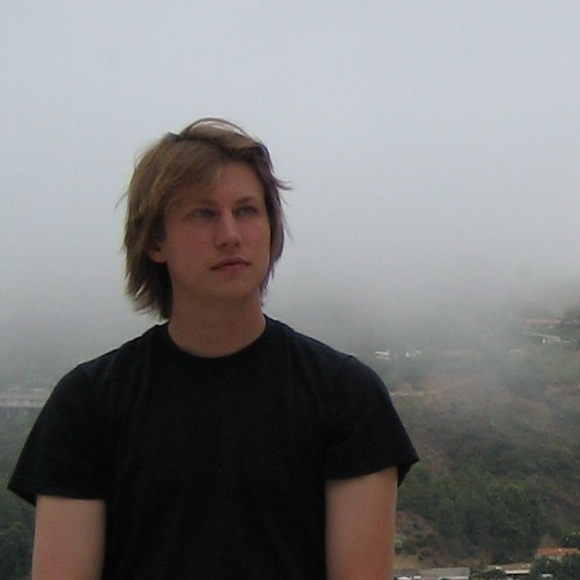
\includegraphics[width=.5\linewidth]{demo_face/jason_02.jpg}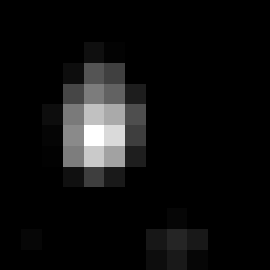
\includegraphics[width=.5\linewidth]{demo_face/face_jason_02.png} \\
  \vspace{.5ex}
  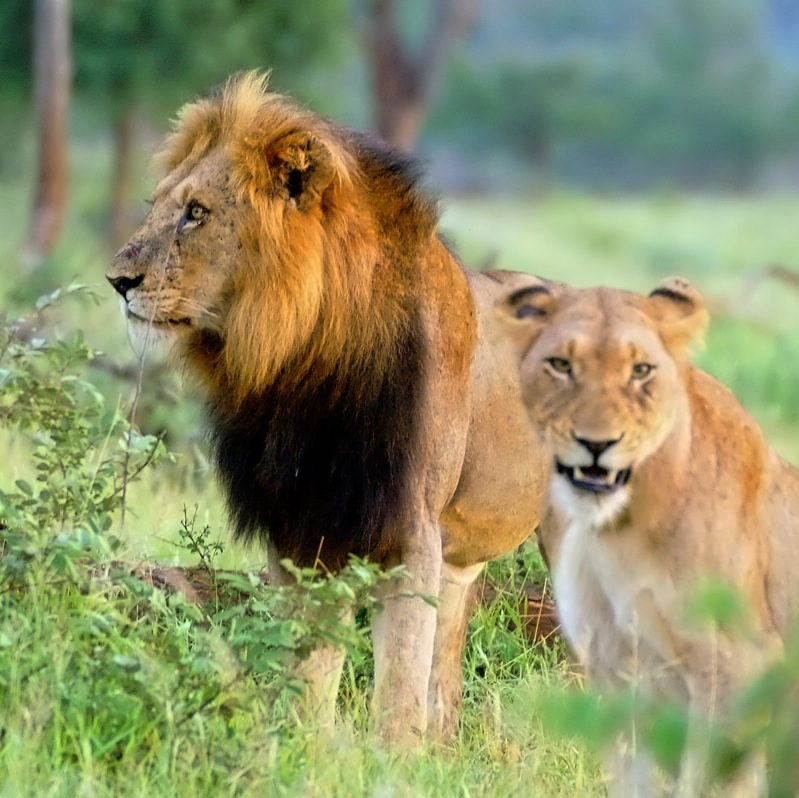
\includegraphics[width=.5\linewidth]{demo_face/lions_arnolouise.jpg}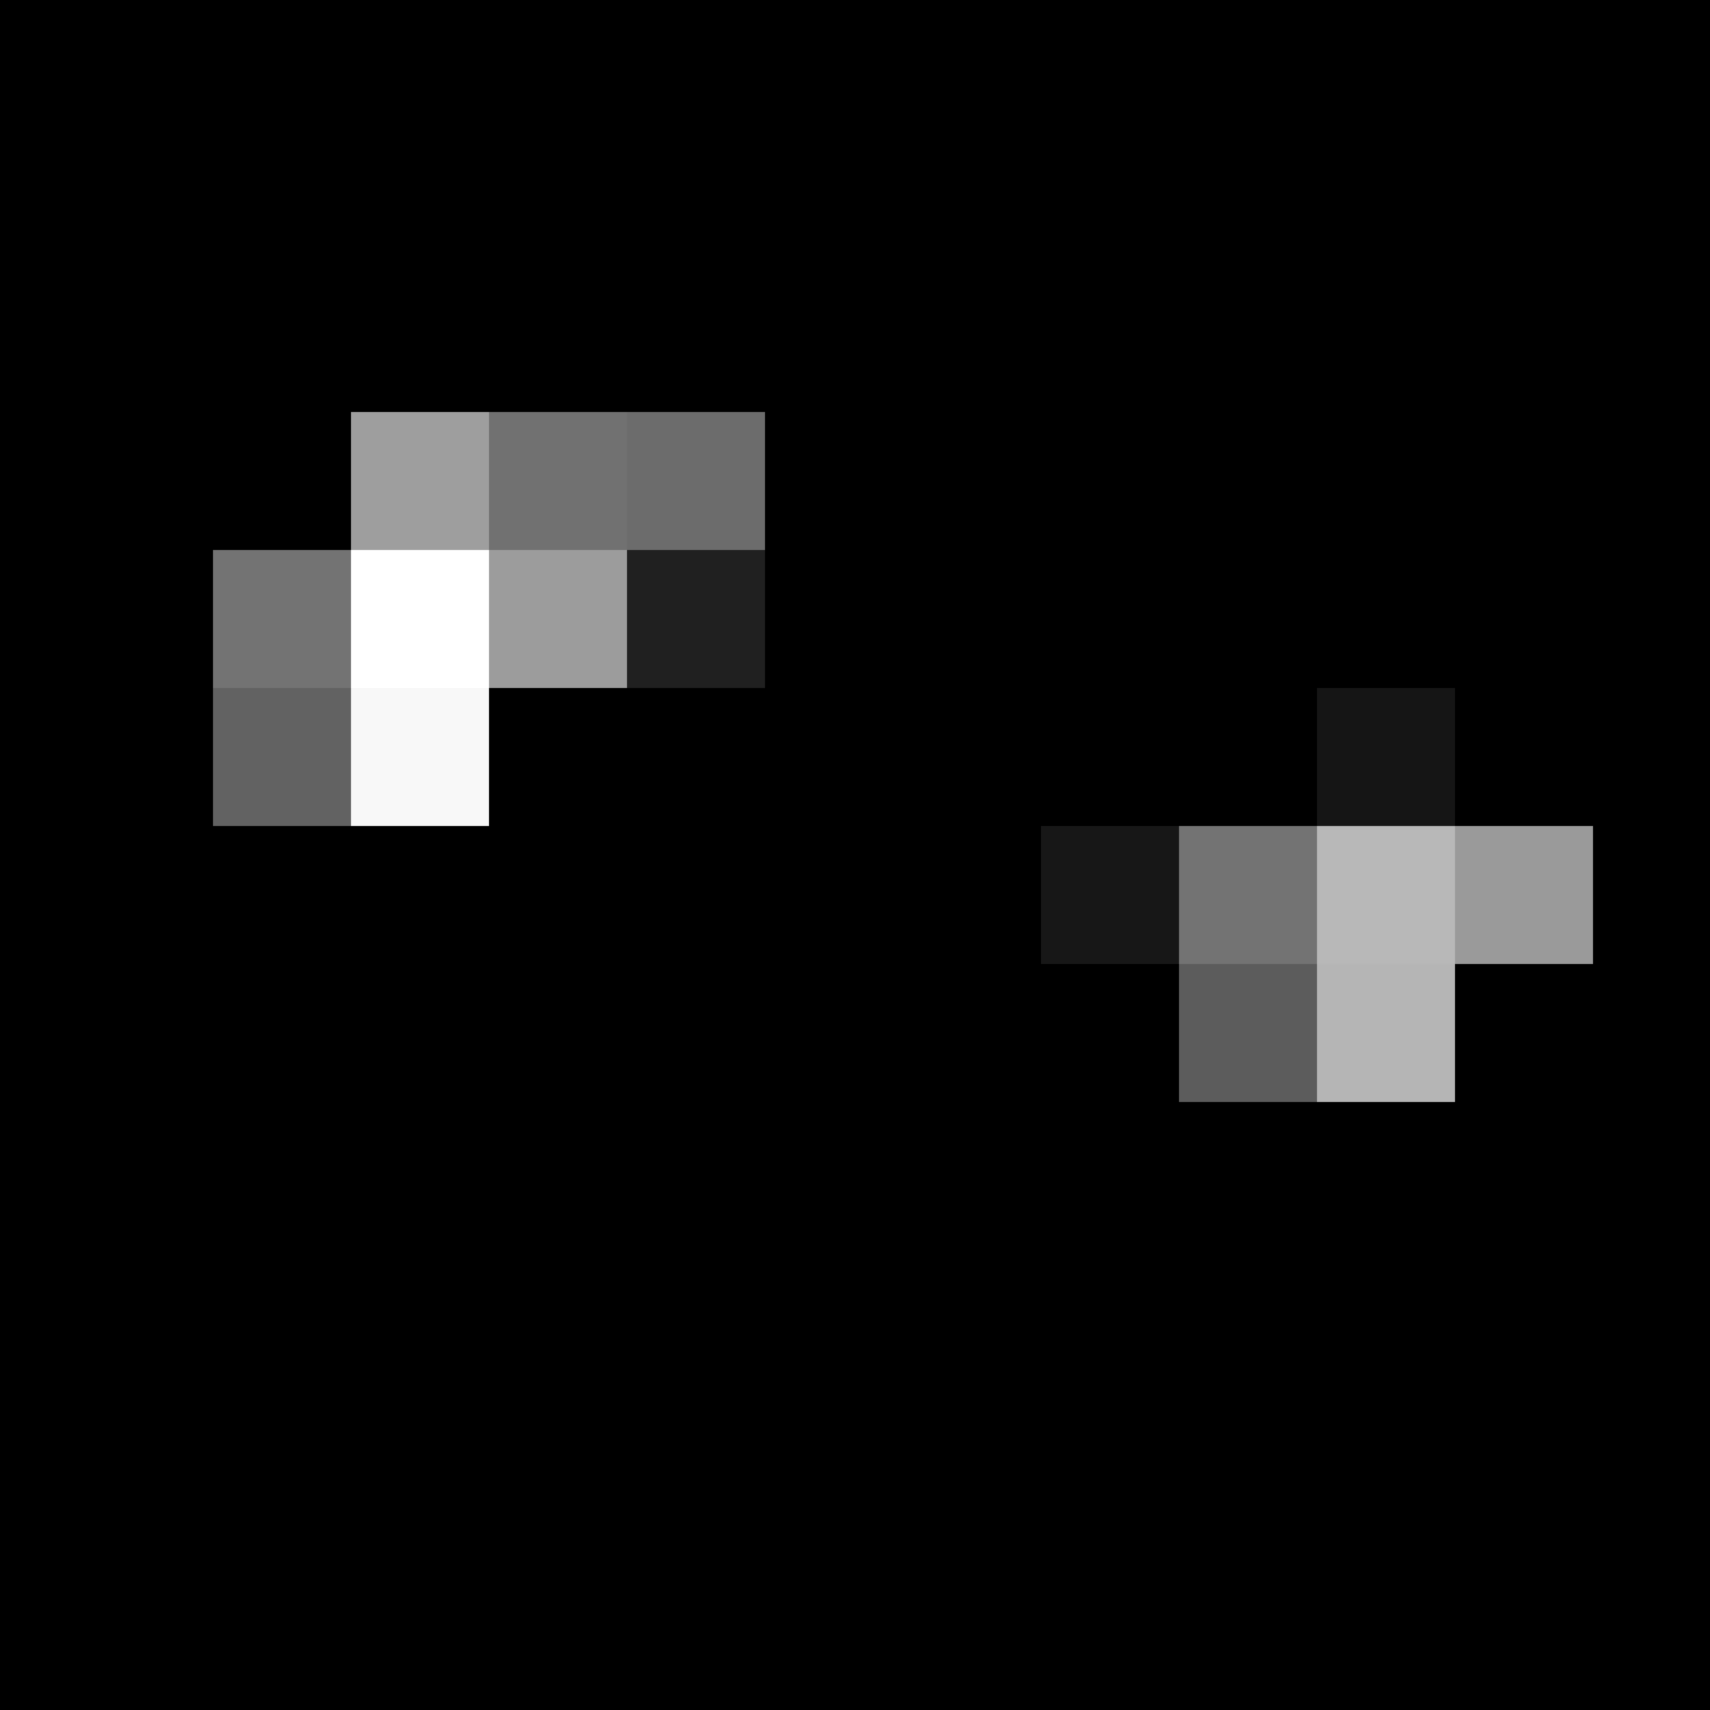
\includegraphics[width=.5\linewidth]{demo_face/face_lions_arnolouise.png}
  \caption{A view of the 13$\times$13 activations of the 151\textsuperscript{st} channel on the \layer{conv5} layer of a deep neural network trained on ImageNet, a dataset that does not contain a face class, but does contain many images with faces. The channel  responds to human and animal faces and is robust to changes in scale, pose, lighting, and context, which can be discerned by a user by actively changing the scene in front of a webcam or by loading static images (e.g. of the lions) and seeing the corresponding response of the unit.
    Photo of lions via Flickr user arnolouise, licensed under CC BY-NC-SA 2.0.
  }
  \figlabel{demo_face}
\end{center}
\vskip -0.2in
\end{figure}

Although this visualization is simple to implement, we find it informative because
all data flowing through the network can be visualized. There is nothing mysterious happening behind the scenes. Because this convnet contains only a single path from input to output, every layer is a bottleneck through which all information must pass en-route to a classification decision. The layer sizes are all small enough that any one layer can easily fit on a computer screen.\footnote{The layer with the most activations is \layer{conv1} which, when tiled, is only 550x550 before adding padding.} So far, we have gleaned several surprising intuitions from using the tool:

%\todo{The first reason is an argument about why it is informative (as the list intro promises)...but the rest are things that we learned by using it, which is a different type of information. One could have argued for the first bullet without using the tool....but the other ones are surprises. I suggest saying ``We find this visualization informative because <list first bullet>. In fact, it taught us many new, surprising things about convnets, including: <bulleted list with the rest of the bullets>''}

\begin{itemize}

%\todo {Our best claim for an important finding that resulted from this demo in the rebuttal was the distributed vs. local representation issue....but that is not mentioned at all in this list (or anywhere in the paper). Consider grabbing that text or rewriting it in a bullet here}

\item One of the most interesting conclusions so far has been that representations on some layers seem to be surprisingly local. Instead of finding distributed representations on all layers, we see, for example, detectors for text, flowers, fruit, and faces on \layer{conv4} and \layer{conv5}. These conclusions can be drawn either from the live visualization or the optimized images (or, best, by using both in concert) and suggest several directions for future research (discussed in \secref{conclusion}).

\item When using direct file input to classify photos from Flickr or Google Images, classifications are often correct and highly confident (softmax probability for correct class near 1). On the other hand, when using input from a webcam, predictions often cannot be correct because no items from the training set are shown in the image. The training set's 1000 classes, though numerous, do not cover most common household objects. Thus, when shown a typical webcam view of a person with no ImageNet classes present, the output has no single high probability, as is expected. Surprisingly, however, this probability vector is noisy and varies significantly in response to tiny changes in the input, often changing merely in response to the noise from the webcam. We might have instead expected unchanging and low confidence predictions for a given scene when no object the network has been trained to classify is present. Plotting the fully connected layers (\layer{fc6} and \layer{fc7}) also reveals a similar sensitivity to small input changes. 

\item Although the last three layers are sensitive to small input changes, much of the lower layer computation is more robust. For example, when visualizing the \layer{conv5} layer, one can find many invariant detectors for faces, shoulders, text, etc. by moving oneself or objects in front of the camera. Even though the 1000 classes contain no explicitly labeled faces or text, the network learns to identify these concepts simply because they represent useful partial information for making a later classification decision. One face detector, denoted \unit{conv5}{151} (channel number 151 on \layer{conv5}), is shown in \figref{demo_face} activating for human and lion faces and in \figref{demo_layers} activating for a cat face. Zhou et al.~\yrcite{zhou-2014-arXiv-object-detectors-emerge} recently observed a similar effect where convnets trained only to recognize different scene types --- playgrounds, restaurant patios, living rooms, etc. --- learn object detectors (e.g. for chairs, books, and sofas) on intermediate layers.

\end{itemize}

The reader is encouraged to try this visualization tool out for him or herself. The code, together with pre-trained models and images synthesized by gradient ascent, can be downloaded at
\url{http://yosinski.com/deepvis}.



\section{Visualizing via Regularized Optimization}
\seclabel{optimization}



The second contribution of this work is introducing several regularization methods to bias images found via optimization toward more visually interpretable examples. While each of these regularization methods helps on its own, in combination they are even more effective. We found useful combinations via a random hyperparameter search, as discussed below.



%\subsection{Regularization methods}
\seclabel{reg_methods}

Formally, consider an image $\x \in \mathbb{R} ^ {C \times H \times W}$, where\ $C = 3$ color channels and the height ($H$) and width ($W$) are both 227 pixels. When this image is presented to a neural network, it causes an activation $a_i(\x)$ for some unit $i$, where for simplicity $i$ is an index that runs over all units on all layers. We also define a parameterized regularization function $R_\theta(\x)$ that penalizes images in various ways.

Our network was trained on ImageNet by first subtracting the per-pixel mean of examples in ImageNet before inputting training examples to the network. Thus, the direct input to the network, $\x$, can be thought of as a zero-centered input.  We may pose the optimization problem as finding an image $\xs$ where

\be
\xs = \argmax_\x(a_i(\x) - R_{\theta}(\x))
\ee

In practice, we use a slightly different formulation. Because we search for $\xs$ by starting at some $\xn$ and taking gradient steps, we instead define the regularization via an operator $r_\theta(\cdot)$ that maps $\x$ to a slightly more regularized version of itself. This latter definition is strictly more expressive, allowing regularization operators $r_\theta$ that are not the gradient of any $R_\theta$.
%\todo{(i.e. regularizers that are non-differentiable)}.
This method is easy to implement within a gradient descent framework by simply alternating between taking a step toward the gradient of $a_i(\x)$ and taking a step in the direction given by $r_\theta$. With a gradient descent step size of $\eta$, a single step in this process applies the update:

\be
\x \leftarrow r_\theta\left(\x + \eta\frac{\partial a_i}{\partial \x}\right) \\
\ee

We investigated the following four regularizations. All are designed to overcome different pathologies commonly encountered by gradient descent without regularization.

% sweep 0
{\bf $L_2$ decay}: A common regularization, $L_2$ decay penalizes large values and is implemented as $r_\theta(\x) =(1 - \theta_{\mathrm{decay}})\cdot\x$. $L_2$ decay tends to prevent a small number of extreme pixel values from dominating the example image. Such extreme single-pixel values neither occur naturally with great frequency nor are useful for visualization. $L_2$ decay was also used by Simonyan et al.~\yrcite{simonyan2013deep-inside-convolutional}.

% sweep 1
{\bf Gaussian blur}: Producing images via gradient ascent tends to produce examples with high frequency information (see Supplementary \secref{high_freq} for a possible reason). While these images cause high activations, they are neither realistic nor interpretable \cite{nguyen-2014-arXiv-deep-neural-networks}. A useful regularization is thus to penalize high frequency information. We implement this as a Gaussian blur step $r_\theta(\x) = \mathrm{GaussianBlur}(\x, \theta_{\mathrm{b\_width}})$. Convolving with a blur kernel is more computationally expensive than the other regularization methods, so we added another hyperparameter $\theta_{\mathrm{b\_every}}$ to allow, for example, blurring every several optimization steps instead of every step. Blurring an image multiple times with a small width Gaussian kernel is equivalent to blurring once with a larger width kernel, and the effect will be similar even if the image changes slightly during the optimization process. This technique thus lowers computational costs without limiting the expressiveness of the regularization. Mahendran \& Vedaldi~\yrcite{mahendran-2014-arXiv-understanding-deep-image} used a penalty with a similar effect to blurring, called \emph{total variation}, in their work reconstructing images from layer codes.
%\footnote{At least one difference is that the Gaussian penalty is isotropic, whereas total variation depends }

% sweep: 3
{\bf Clipping pixels with small norm}: The first two regularizations suppress high amplitude and high frequency information, so after applying both, we are left with an $\xs$ that contains somewhat small, somewhat smooth values. However, $\xs$ will still tend to contain non-zero pixel values everywhere. Even if some pixels in $\xs$ show the primary object or type of input causing the unit under consideration to activate, the gradient with respect to all other pixels in $\xs$ will still generally be non-zero, so these pixels will also shift to show some pattern as well, contributing in whatever small way they can to ultimately raise the chosen unit's activation. We wish to bias the search away from such behavior and instead show only the main object, letting other regions be exactly zero if they are not needed. We implement this bias using an $r_\theta(\x)$ that computes the norm of each pixel (over red, green, and blue channels) and then sets any pixels with small norm to zero. The threshold for the norm, $\theta_{\mathrm{n\_pct}}$, is specified as a percentile of all pixel norms in $\x$.

% sweep: 2
{\bf Clipping pixels with small contribution}: Instead of clipping pixels with small norms, we can try something slightly smarter and clip pixels with small \emph{contributions} to the activation. One way of computing a pixel's contribution to an activation is to measure how much the activation increases or decreases when the pixel is set to zero; that is, to compute the contribution as $|a_i(\x) - a_i(\x_{-j})|$, where $\x_{-j}$ is $\x$ but with the $j^{th}$ pixel set to zero. This approach is straightforward but prohibitively slow, requiring a forward pass for every pixel. Instead, we approximate this process by linearizing $a_i(\x)$ around $\x$, in which case the contribution of each dimension of $\x$ can be estimated as the elementwise product of $\x$ and the gradient. We then sum over all three channels and take the absolute value, computing  $\left|\sum_c \x \circ \nabla_\x a_i(\x)\right|$. We use the absolute value to find pixels with small contribution in either direction, positive or negative. While we could choose to keep the pixel transitions where setting the pixel to zero would result in a large activation increase, these shifts are already handled by gradient ascent, and here we prefer to clip only the pixels that are deemed not to matter, not to take large gradient steps outside the region where the linear approximation is most valid. We define this $r_\theta(\x)$ as the operation that sets pixels with contribution under the $\theta_{\mathrm{c\_pct}}$ percentile to zero.

%\todo{TODO: As noted in \cite{goodfellow-2014-arXiv-explaining-and-harnessing-adversarial}, small changes * many....}

%\begin{figure*}[ht]
%\vskip 0.2in
%\begin{center}
%\centerline{\includegraphics[width=1\linewidth]{demo_layers/demo_layers.jpg}}
%\caption{}
%\figlabel{demo_layers}
%\end{center}
%\vskip -0.2in
%\end{figure*}

%\subsection{Results and Discussion}
\seclabel{results}

\begin{figure}[!th]
%\vskip -0.4in
\begin{center}
\centerline{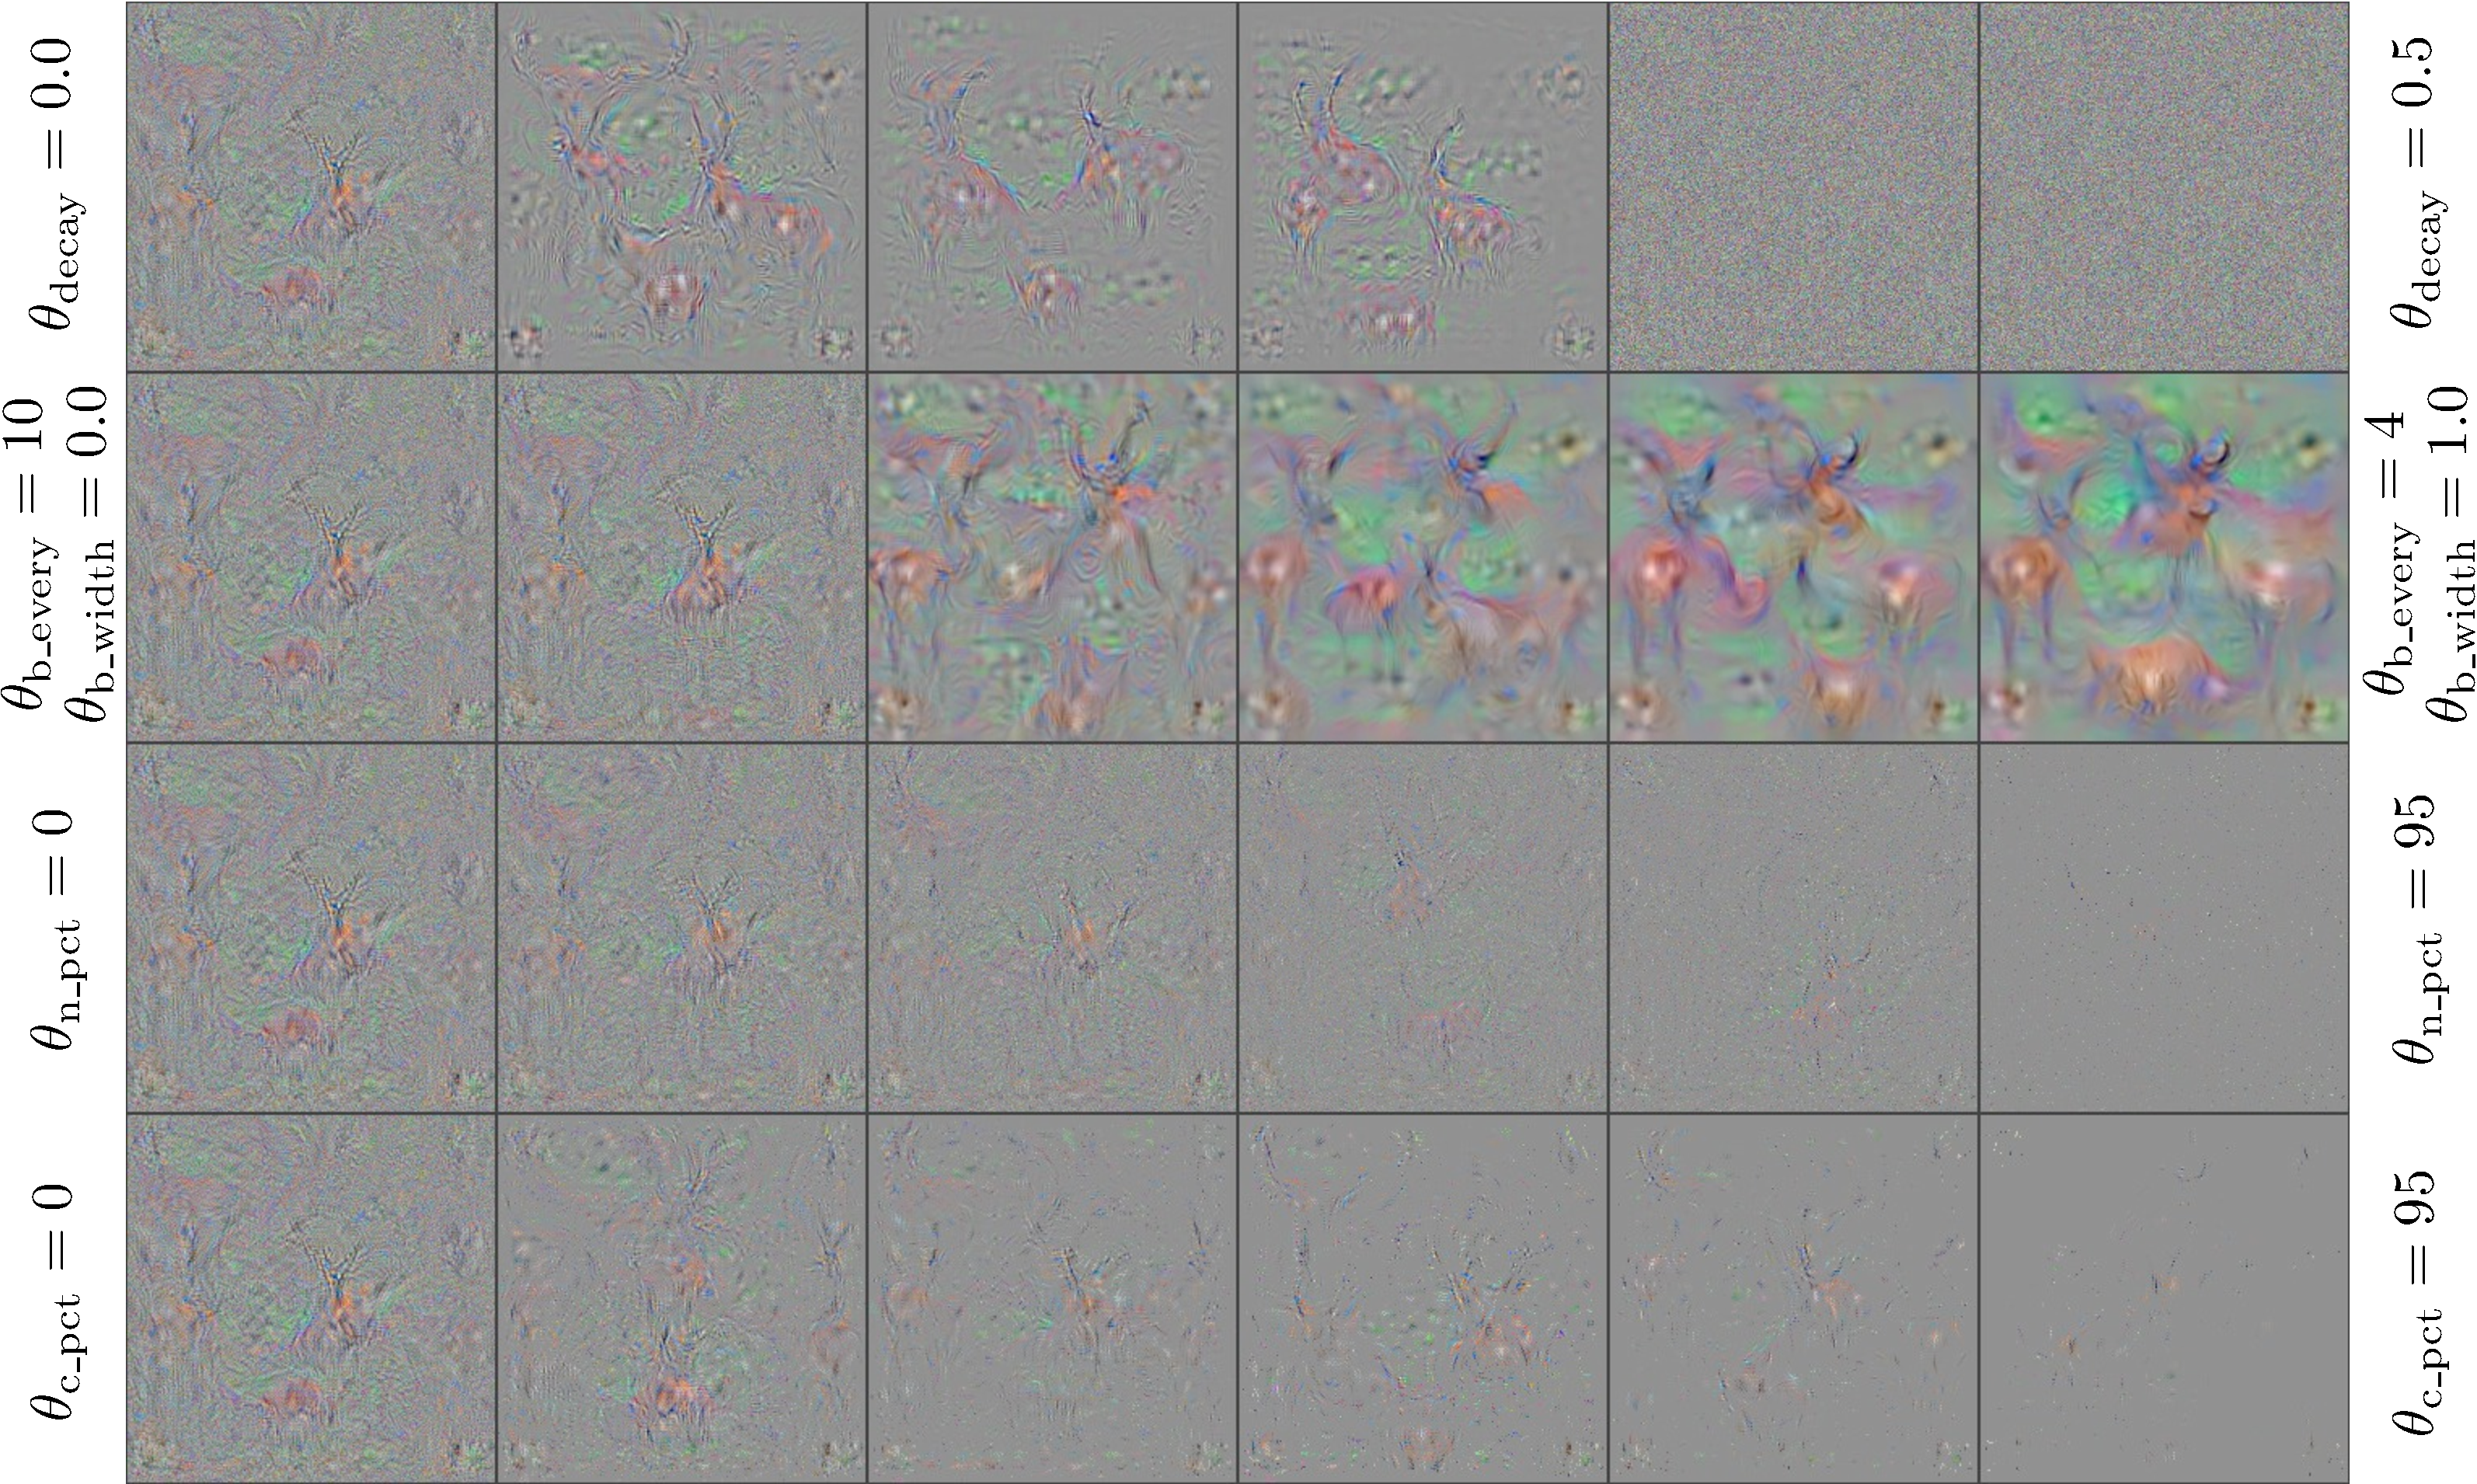
\includegraphics[width=1.0\linewidth]{regularization_sweep_crop.pdf}}
\caption{The effects of each regularization method from \secref{optimization} when used individually. Each of the four rows shows a linear sweep in hyperparameter space from no regularization (left) to strong regularization (right).
  When applied too strongly, some regularizations cause the optimization to fail (e.g. $L_2$ decay, top row) or the images to be less interpretable (small norm and small contribution clipping, bottom two rows). For this reason, a random hyperparameter search was useful for finding joint hyperparameter settings that worked well together (see \figref{vis_fc8}).
Best viewed electronically, zoomed in.
}
\figlabel{regularization_sweep}
\end{center}
%\vskip -0.9in
\end{figure}

If the above regularization methods are applied individually, they are
somewhat effective at producing more interpretable images; \figref{regularization_sweep} shows the effects of each individual hyperparameter.
However, preliminary experiments uncovered that their combined
effect produces better visualizations. To pick a reasonable set of
hyperparameters for all methods at once, we ran a random
hyperparameter search of 300 possible combinations and settled on four
that complement each other well. The four selected combinations are
listed in \tabref{paramTable} and optimized images using each are shown for the ``Gorilla'' class output unit in \figref{vis_fc8}. Of the four, some show high
frequency information, others low frequency; some contain dense
pixel data, and others contain only sparse outlines of important
regions.
%\todo{makes it sound like we have dozens...but you list four descriptions for four hyperparam settings. Instead say ``One (top right) doe x, another (bottom right) does y, etc.''}
We found the version in the lower-left quadrant to be the best single set of hyperparameters, but often greater intuition can
be gleaned by considering all four at once.
\figref{vis_all} shows the optimization results computed for a selection of units on all layers. A single image for every filter of all five convolutional layers is shown in Supplementary \figref{layer_montages}. Nine images for each filter of all layers, including each of the 1000 ImageNet output classes, can be viewed at \url{http://yosinski.com/deepvis}.
%\todo{Nothing in here mentions the other classes of Fig 4 (we only mention the gorilla class), and nothing reports any results learned by viewing these visualizations}

\begin{table}[t]
\caption{Four hyperparameter combinations that produce different styles of recognizable images. We identified these four after reviewing images produced by 300 randomly selected hyperparameter combinations. From top to bottom, they are the hyperparameter combinations that produced the top-left, top-right, bottom-left, and bottom-right Gorilla class visualizations, respectively, in \figref{vis_fc8}. The third row hyperparameters produced most of the visualizations for the other classes in \figref{vis_fc8}, and all of those in \figref{vis_all}.
}
\tablabel{boost}
\begin{center}
\begin{tabular}{|c|c|c|c|c|}
  \hline
  $\theta_{\mathrm{decay}}$ & $\theta_{\mathrm{b\_width}}$ & $\theta_{\mathrm{b\_every}}$ & $\theta_{\mathrm{n\_pct}}$ & $\theta_{\mathrm{c\_pct}}$  \\
  \hline
    0    &   0.5   &     4    &    50    &    0 \\
    0.3  &    0    &     0    &    20    &    0 \\
  0.0001 &   1.0   &     4    &     0    &    0 \\
    0    &   0.5   &     4    &     0    &   90 \\
\hline
\end{tabular}
\end{center}
\tablabel{paramTable}
\end{table}


%\todo{TODO: compare to Karen: much better.}
\begin{figure*}[!ht]
\vskip -0.2in
\begin{center}
\centerline{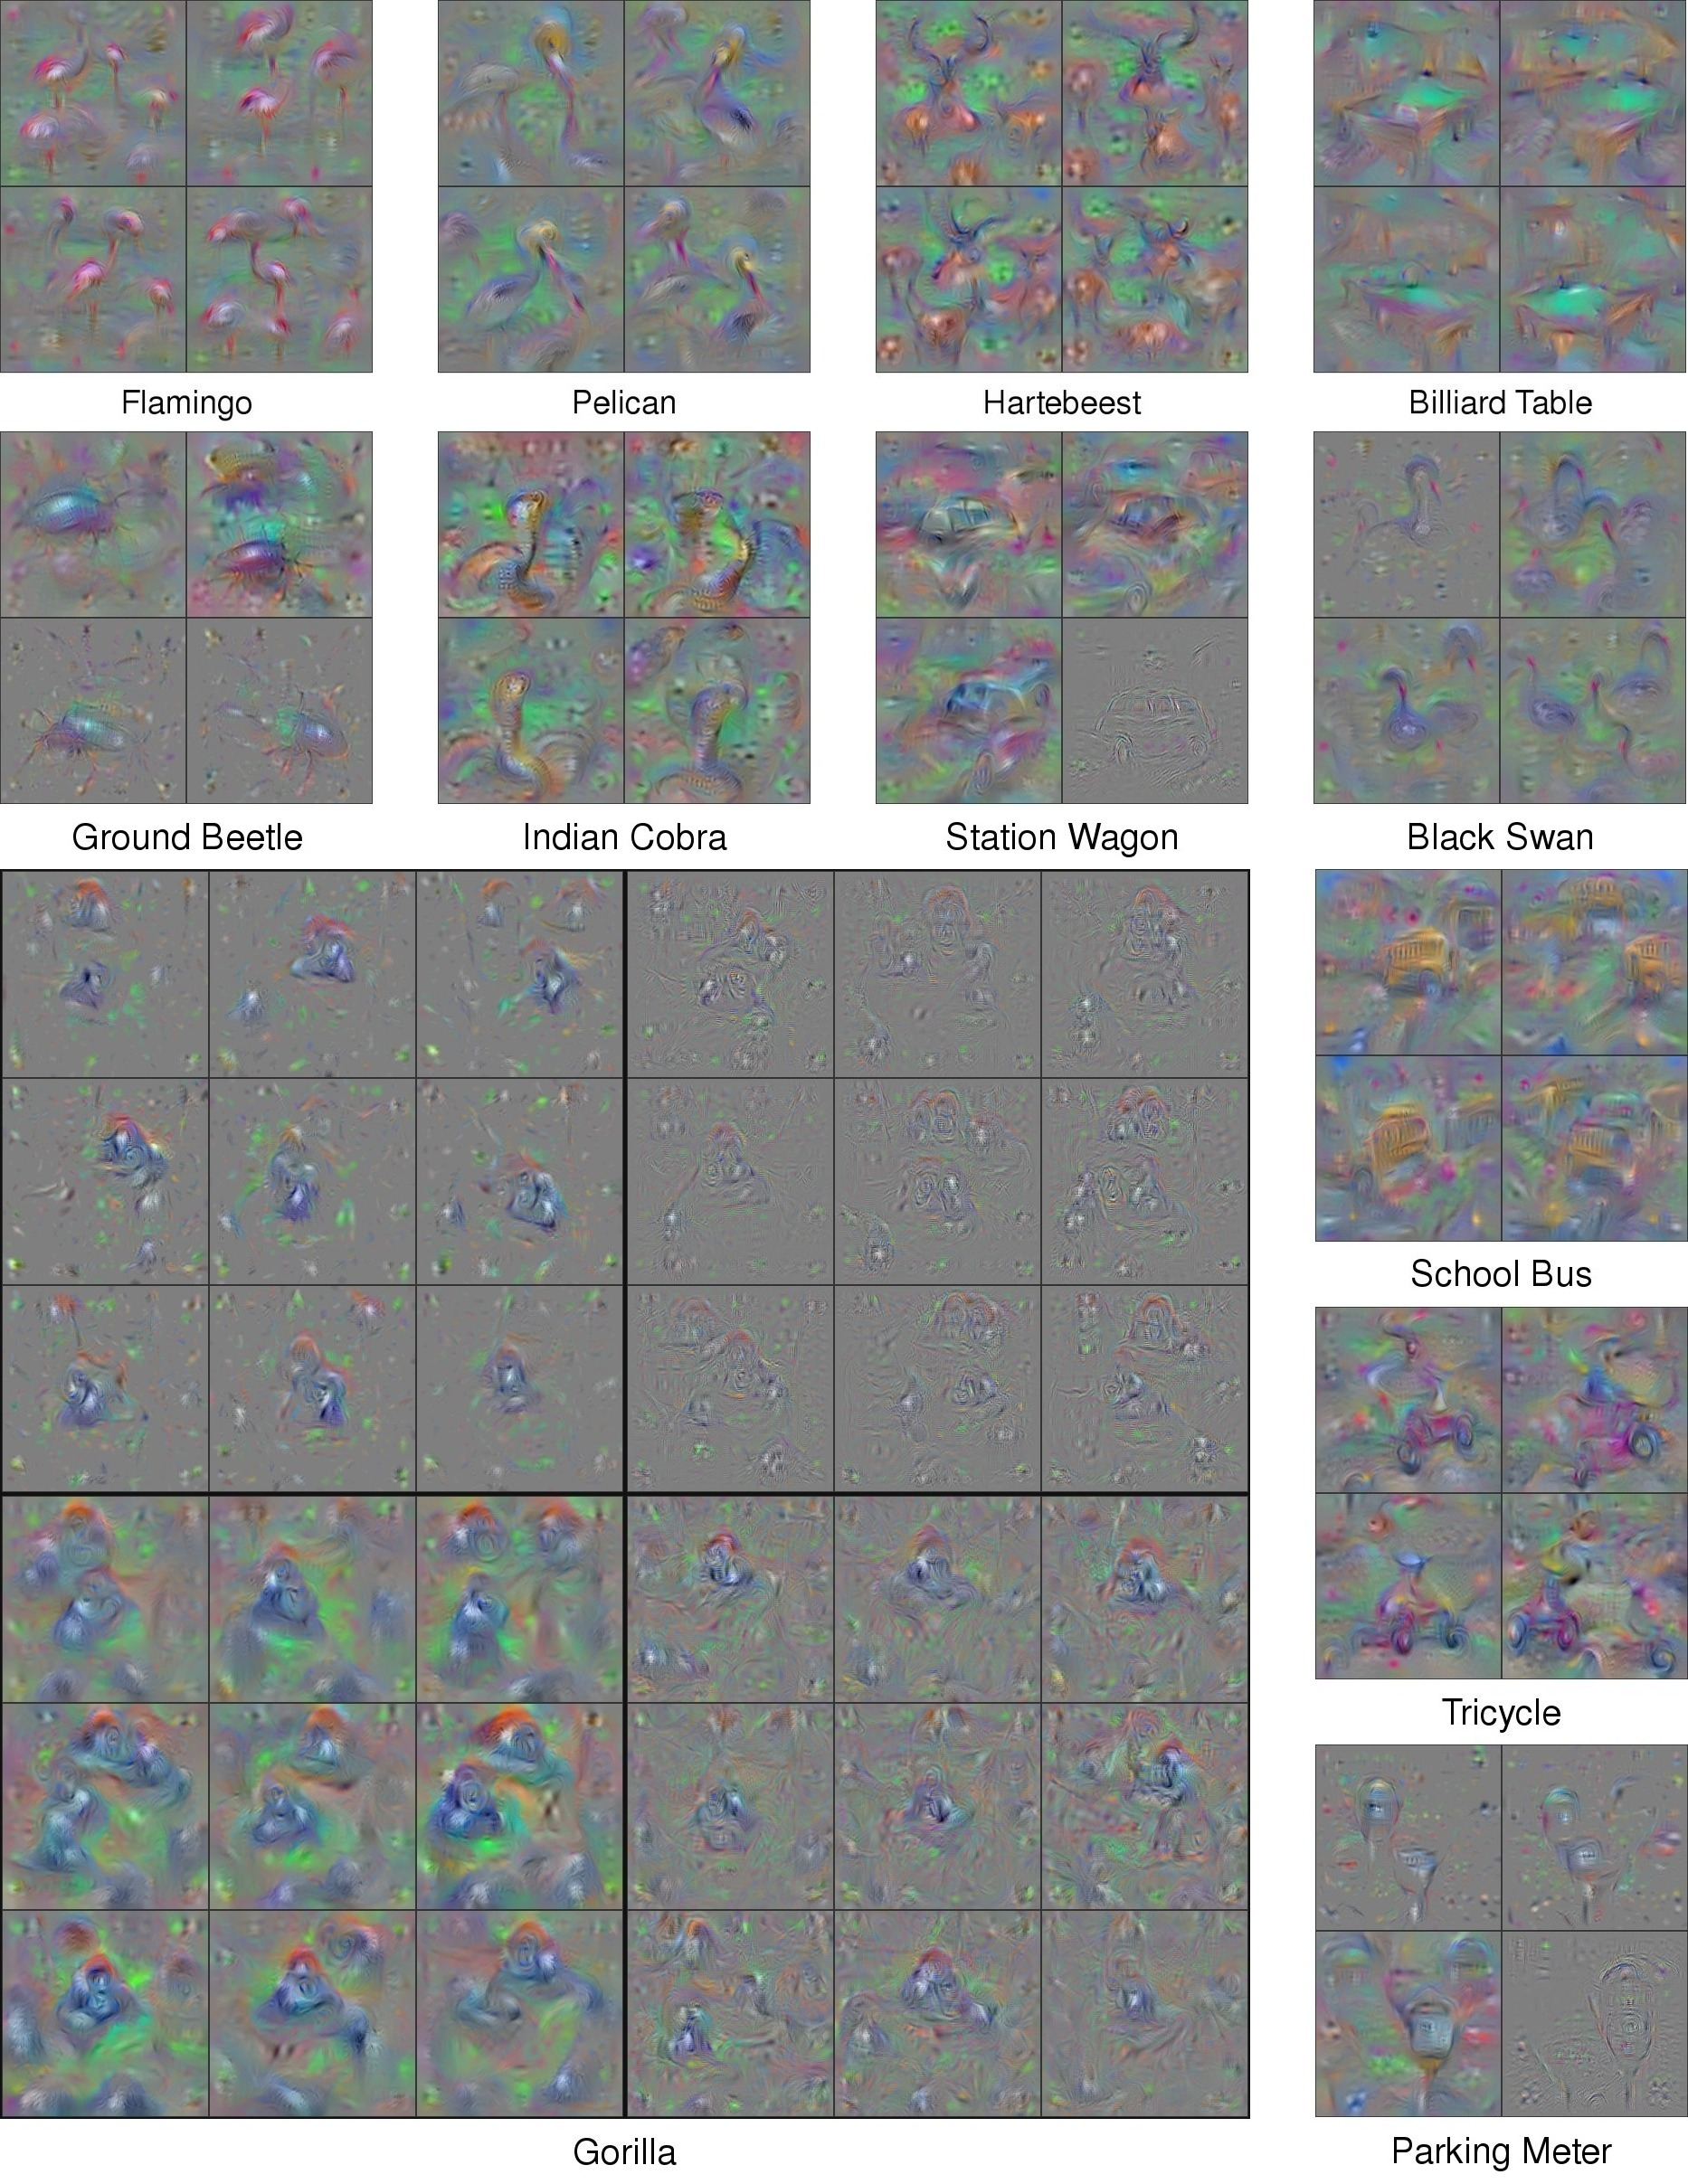
\includegraphics[width=.95\linewidth]{fc8-visualized.jpg}}
\vskip -0.2in
\caption{Visualizations of the preferred inputs for different class units on layer \layer{fc8}, the 1000-dimensional output of the network just before the final softmax. In the lower left are 9 visualizations each (in 3$\times$3 grids) for four different sets of regularization hyperparameters for the Gorilla class (\tabref{paramTable}). For all other classes, we have selected four interpretable visualizations produced by our regularized optimization method. We chose the four combinations of regularization hyperparameters by performing a random hyperparameter search and selecting combinations that complement each other. For example, the lower left quadrant tends to show lower frequency patterns, the upper right shows high frequency patterns, and the upper left shows a sparse set of important regions.  Often greater intuition can be gleaned by considering all four at once. In nearly every case, we have found that one can guess what class a neuron represents by viewing sets of these optimized, preferred images. Best viewed electronically, zoomed in.
  %\todo{more big picture payoff?}
}
\figlabel{vis_fc8}
\end{center}
\vskip -0.9in
\end{figure*}

\begin{figure*}[!ht]
\vskip 0.2in
\begin{center}
\centerline{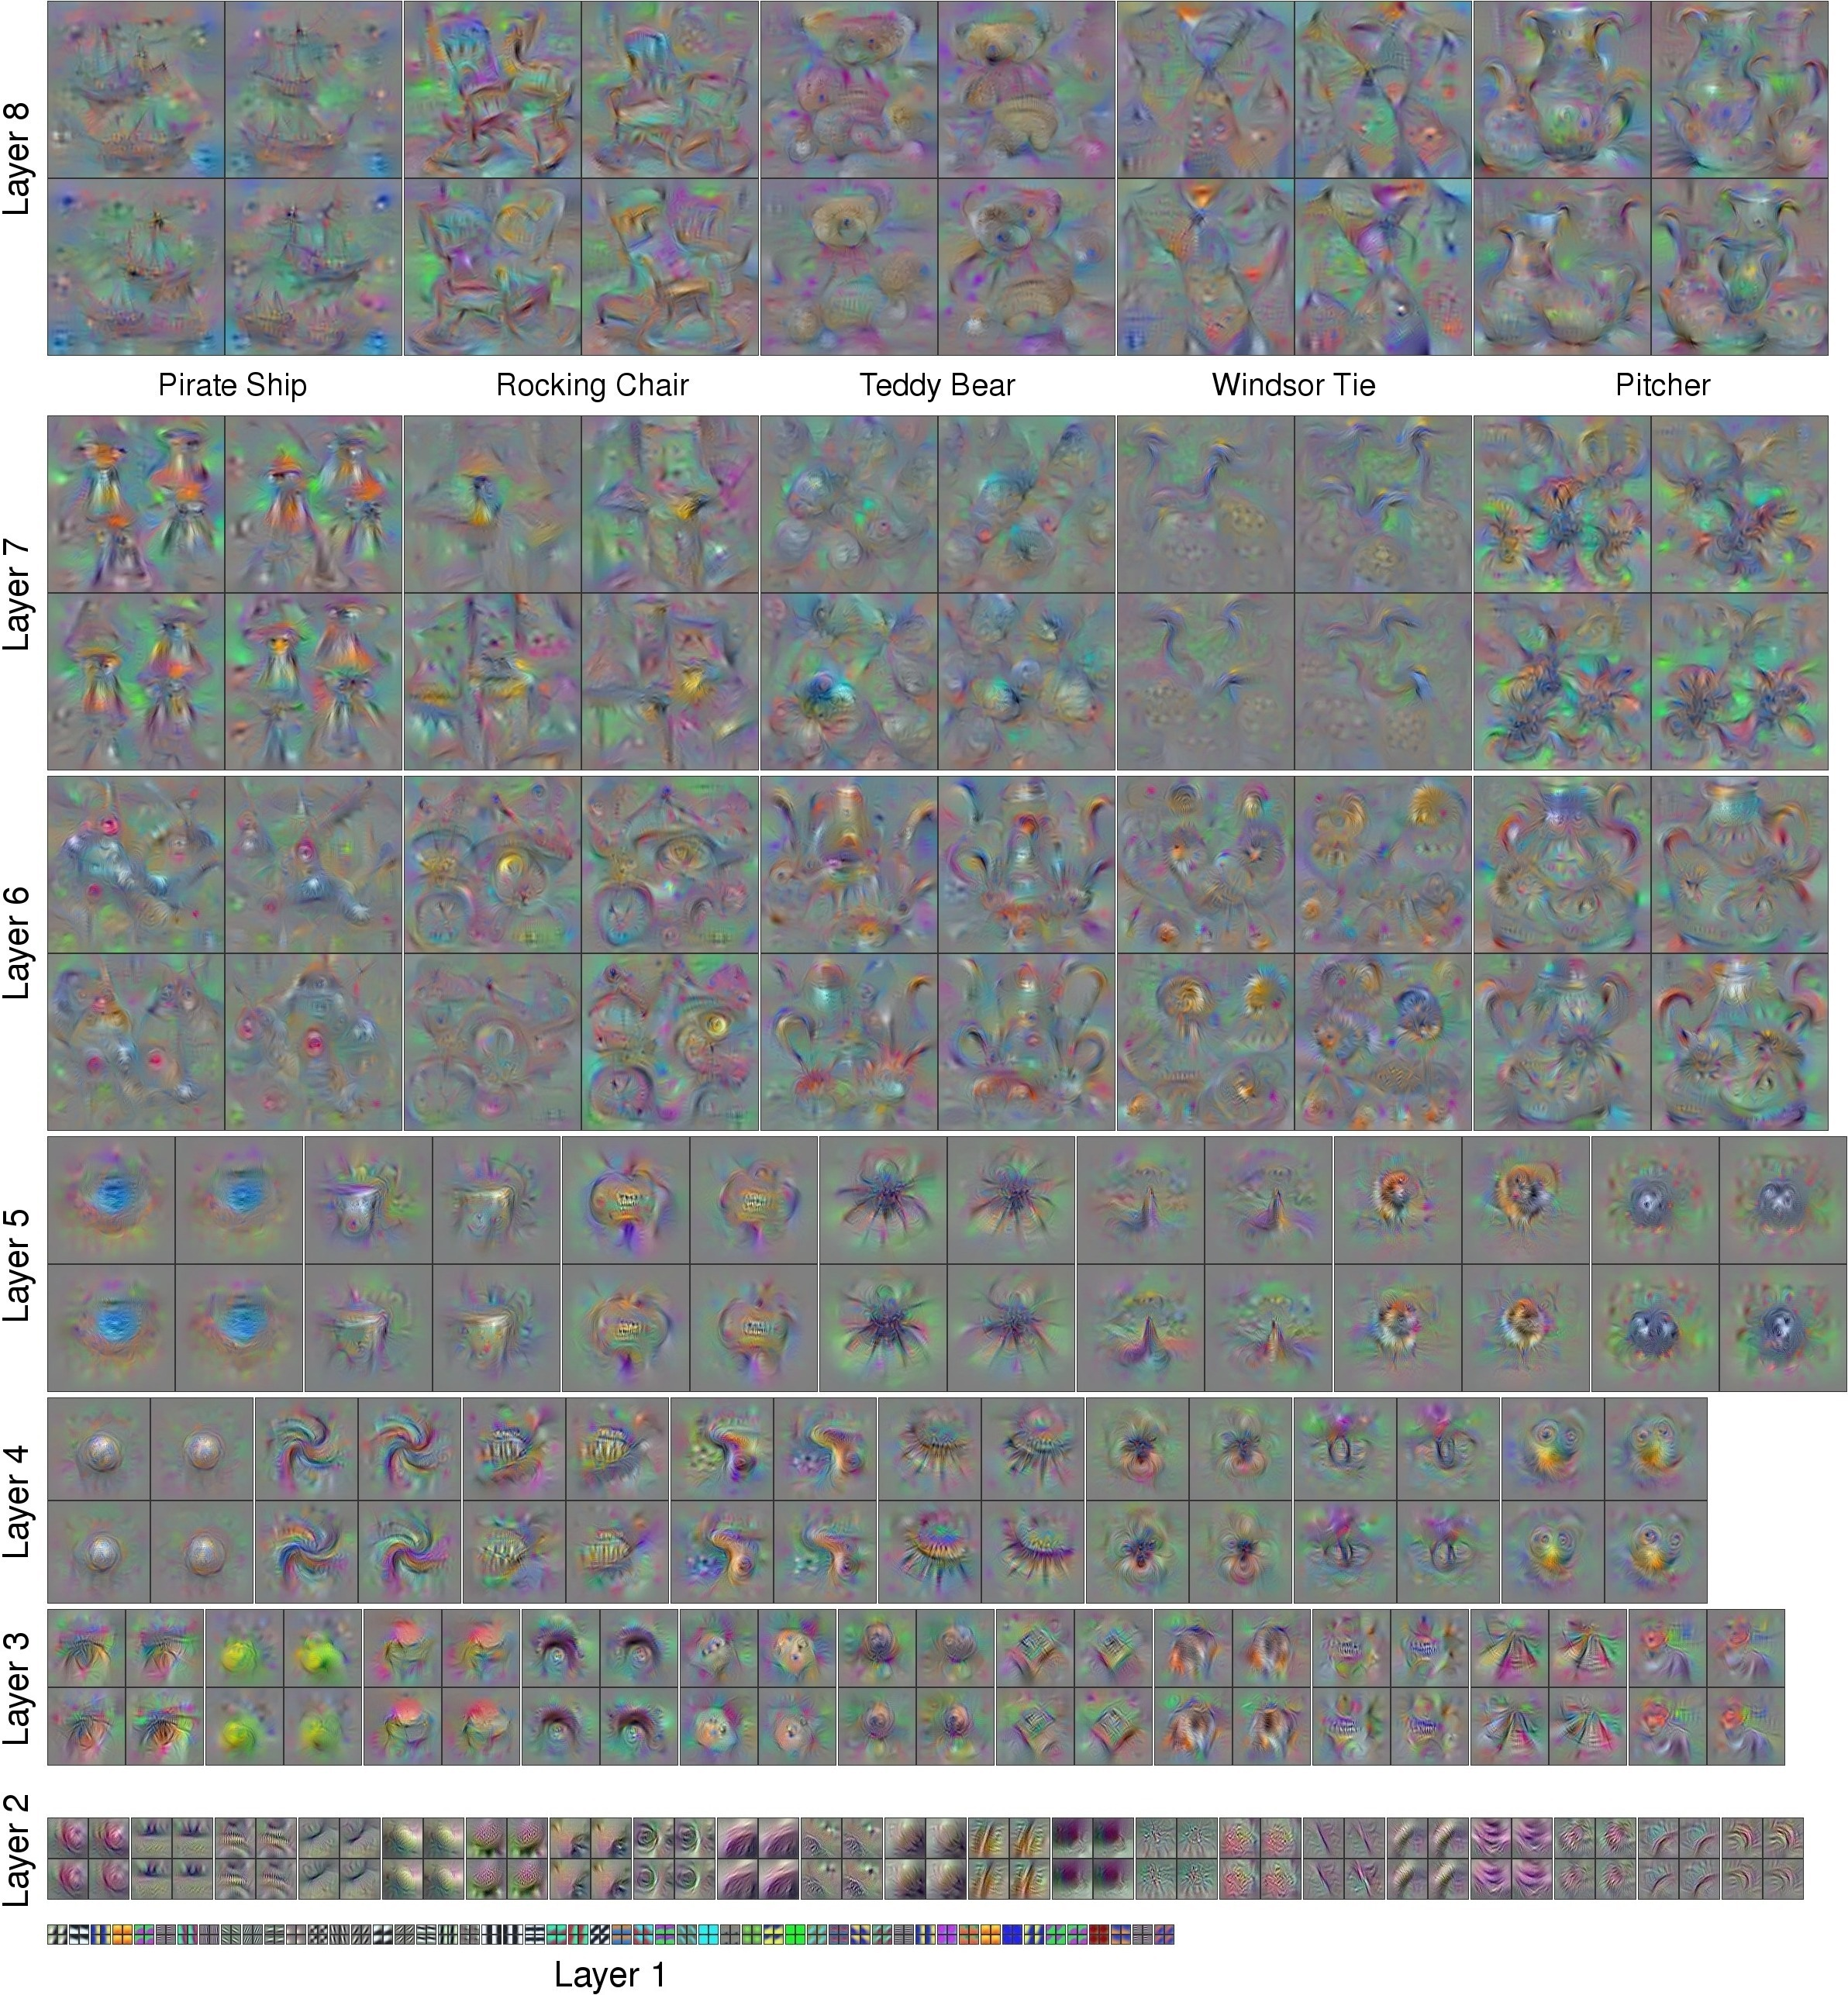
\includegraphics[width=1\linewidth]{all_layers.jpg}}
\caption{Visualization of example features of eight layers of a deep, convolutional neural network. The images reflect the true sizes of the features at different layers. In each layer, we show visualizations from 4 random gradient descent runs for each channel. While these images are hand picked to showcase the diversity and interpretability of the visualizations, one image for each filter of all five convolutional layers is shown in Figure S1 in supplementary information. One can recognize important features of objects at different scales, such as edges, corners, wheels, eyes, shoulders, faces, handles, bottles, etc. The visualizations show the increase in complexity and variation on higher layers, comprised of simpler components from lower layers. The variation of patterns increases with increasing layer number, indicating that increasingly invariant representations are learned. In particular, the jump from Layer 5 (the last convolution layer) to Layer 6 (the first fully-connected layer) brings about a large increase in variation. Best viewed electronically, zoomed in.
%  from thus help document that DNNs learn \todo{insert what we want to say..hierarchal assemblies of features?}\todo{more big picture payoff? more just saying that it works and is the best so far?} 
}
\figlabel{vis_all}
\end{center}
\vskip -0.2in
\end{figure*}



%\vspace*{-.1em}
\section{Discussion and Conclusion}
\seclabel{conclusion}
%\vspace*{-.1em}

We have introduced two visual tools for aiding in the interpretation
of trained neural nets.
%To enable the widest possible community to benefit from these tools, we have released the source code for both tools online.
Intuition gained from these tools may prompt ideas for improved methods and future research. Here we discuss several such ideas.

%The first tool allows users to interact with a
%convnet using static images or images from a webcam. The user can see how every neural unit in a DNN responds to these different inputs.
The interactive tool reveals that representations on later convolutional layers tend to be somewhat local, where channels correspond to specific, natural parts (e.g. wheels, faces) instead of being dimensions in a completely distributed code. That said, not all features correspond to natural parts, raising the possibility of a different decomposition of the world than humans might expect. These visualizations suggest that further study into the exact nature of learned representations --- whether they are local to a single channel or distributed across several --- is likely to be interesting (see Zhou et al.~\yrcite{zhou-2014-arXiv-object-detectors-emerge} for work in this direction). The locality of the representation also suggests that during transfer learning, when new models are trained atop the \layer{conv4} or \layer{conv5} representations, a bias toward sparse connectivity could be helpful because it may be necessary to combine only a few features from these layers to create important features at higher layers.

The second tool --- new regularizations that enable improved, interpretable, optimized visualizations of learned features --- will help researchers and practitioners understand, debug, and improve their models. The visualizations also reveal a new twist in an ongoing story. Previous studies
have shown that discriminative networks can easily be fooled or hacked by the addition of certain structured
noise in image space \cite{szegedy2013intriguing-properties-of-neural,nguyen-2014-arXiv-deep-neural-networks}.
An oft-cited reason for this property is that discriminative training leads networks
%does not require networks to learn a density $p(x)$ over
%their whole input space $x$, rather, only a conditional density $p(y|x)$ for a label space $y$ is needed.
%In other words, discriminative networks may
to ignore non-discriminative information in their input, e.g. learning to detect jaguars by matching the unique spots on their fur while ignoring the fact that they have four legs. For this reason it has been seen as a hopeless endeavor to create a generative model in which one randomly samples an $x$ from a broad distribution on the space of all possible images
%\todo{\footnote{\todo{I think I screwed this sentence up, because I did not really know what you meant. Many readers will not follow this if we use p(x) in the sentence...we should try to describe it more intuitively}}}
and then iteratively transforms $x$ into a recognizable image by moving it to a region that satisfies both a prior $p(x)$ and posterior $p(y|x)$ for some class label $y$.
%, and where the image is recognizable as of class $y$.
Past attempts have largely supported this view by producing unrealistic images using this method \cite{nguyen-2014-arXiv-deep-neural-networks,simonyan2013deep-inside-convolutional}.

However, the results presented here suggest an alternate possibility: the previously used priors may simply have been too weak (see \secref{high_freq} for one hypothesis of why a strong $p(x)$ model is needed). With the careful design or learning of a $p(x)$ model that biases toward realism,
one may be able to harness
the large number of parameters present in a discriminately learned $p(y|x)$ model
%\todo{learned by a DNN trained with supervised learning (i.e. a discriminative model)}
to generate realistic images by enforcing probability under both models simultaneously.
Even with the simple, hand-coded $p(x)$ models we use in this paper as regularizers, complex dependencies between distant pixels already arise (cf. the beetles with structure spanning over 100 pixels in \figref{vis_fc8}). This implies that the discriminative parameters also contain significant ``generative'' structure from the
training dataset; that is, the parameters encode
not only the jaguar's spots, but to some extent also its four legs.
%a surprisingly large amount t implies that more structure of the dataset is present in the descriminative parameters.
With better, learned probabilistic models over the input and activations of higher layers, much more structure may be apparent. Work by Dai et al.~\yrcite{dai-2015-ICLR-generative-modeling-of-convolutional} shows some interesting results in this direction.
%It seems that previous approaches may simply have been disadvantaged by having too weak a model for $p(x)$; 
%results could be further improved with an even stronger $p(x)$ model may be needed.
%\todo{do you mean what I changed this to, that an even stronger model informed by the S1 hypothesis would make things even better, or do you simply mean that SI provides a hypothesis for why *such* strong natural image regularizers are necessary?}
While the images generated in this paper are far from being photo-realistic, they do suggest that
transferring discriminatively trained parameters to generative models --- opposite the direction of the usual unsupervised pretraining approach --- may be a fruitful area for further investigation.

%These are a few ideas for next steps based on our use to date of these two tools for understanding deep neural networks. However, the best ideas that these tools will produce may well come from other researchers interacting with and visualizing their own models.
%, and using these tools in ways we have not yet imagined.

% OR SOMETHING LIKE THIS
%Such techniques for illuminating the inner workings of deep neural networks should improve our ability to understand individual, trained DNNs, as well as improve the iterative process of developing more powerful models and techniques for training future generations of deep neural networks.
%
%Exciting new directions for research.





\section*{Acknowledgments} 

The authors would like to thank the NASA Space Technology Research Fellowship (JY) for funding, Wendy Shang, Yoshua Bengio, Brian Cheung, and Andrej Karpathy for helpful discussions, and Freckles the cat for her feline countenance.





{
  \small
\bibliography{bibdesk}
\bibliographystyle{icml2015}
}



\clearpage

% Supplementary Information hacks from http://jshodges.com/index.php?qs=kb_001
% For section headers starting with S
\renewcommand{\thesection}{S\arabic{section}}
\renewcommand{\thesubsection}{\thesection.\arabic{subsection}}

\newcommand{\beginsupplementary}{%
        \setcounter{table}{0}
        \renewcommand{\thetable}{S\arabic{table}}%
        \setcounter{figure}{0}
        \renewcommand{\thefigure}{S\arabic{figure}}%
        \setcounter{section}{0}
     }

\beginsupplementary

%\renewcommand{\titl}{Supplementary Information For:\\Understanding Neural Networks Through Deep Visualization}

% The \icmltitle you define below is probably too long as a header.
% Therefore, a short form for the running title is supplied here:
\icmltitlerunning{\suptitlrunning}

\twocolumn[
  \icmltitle{\suptitl}

% It is OKAY to include author information, even for blind
% submissions: the style file will automatically remove it for you
% unless you've provided the [accepted] option to the icml2015
% package.
\icmlauthor{Jason Yosinski}{yosinski@cs.cornell.edu}
%\icmladdress{Cornell University}
\icmlauthor{Jeff Clune}{jeffclune@uwyo.edu}
%\icmladdress{University of Wyoming}
\icmlauthor{Anh Nguyen}{anguyen8@uwyo.edu}
%\icmladdress{University of Wyoming}
\icmlauthor{Thomas Fuchs}{fuchs@caltech.edu}
%\icmladdress{Jet Propulsion Laboratory, California Institute of Technology}
\icmlauthor{Hod Lipson}{hod.lipson@cornell.edu}
%\icmladdress{Cornell University}

% You may provide any keywords that you 
% find helpful for describing your paper; these are used to populate 
% the "keywords" metadata in the PDF but will not be shown in the document
\icmlkeywords{convolutional neural networks, neural networks, visualization}

\vskip 0.3in
]

%\maketitle



\section{Why are gradient optimized images dominated by high frequencies?}
\seclabel{high_freq}

In the main text we mentioned that images produced by gradient ascent to maximize the activations of neurons in convolutional networks tend to be dominated by high frequency information (cf.  the left column of \figref{regularization_sweep}). One hypothesis for why this occurs centers around the differing statistics of the activations of channels in a convnet. The \layer{conv1} layer consists of blobs of color and oriented Gabor edge filters of varying frequencies. The average activation values (after the rectifier) of the edge filters vary across filters, with low frequency filters generally having much higher average activation values than high frequency filters. In one experiment we observed that the average activation values of the five lowest frequency edge filters was 90 versus an average for the five highest frequency filters of 5.4, a difference of a factor of 17 (manuscript in preparation)\footnote{Li, Yosinski, Clune, Song, Hopcroft, Lipson. 2015. How similar are features learned by different deep neural networks? In preparation.}\textsuperscript{,}\footnote{Activation values are averaged over the ImageNet validation set, over all spatial positions, over the channels with the five \{highest, lowest\} frequencies, and over four separately trained networks.}. The activation values for blobs of color generally fall in the middle of the range.
This phenomenon likely arises for reasons related to the $1/f$ power spectrum of natural images in which low spatial frequencies tend to contain higher energy than high spatial frequencies \citep{torralba-2003-Network-statistics-of-natural-image}.


% - on conv1 low freq filters have larger response, high freq smaller response (give numbers, (unpublished results))
%     From highest activation -> lowest activation figure in   local_distrib/nips
%     octave:1> mean([84 83.5 82.4 81.7 77.4     130.3 118.1 99.5 84.1 60.8    108.6 107.4 95 72.1 61.1     109.6 102.3 88.5 82.0 76.7])
%     ans =  90.255
%     octave:2> mean([4.4 4.7 4.7 5 5.2     4.6 5.4 5.6 5.8 6.0     4.5 5.9 6.4 5.5 5.6     4.9 5.7 6.3 6.3 6.3])
%     ans =  5.4400
% - thus any features in conv2 that employ information from conv1 filters will have higher weights to the smaller activations
% - this may occur on other layers too


%Regardless of the exact reason the phenomenon arises,

Now consider the connections from the \layer{conv1} filters to a single unit on \layer{conv2}.
%, consider the connections from units on the next layer, \layer{conv2}, to the \layer{conv1} units.
In order to merge information from both low frequency and high frequency \layer{conv1} filters, the connection weights from high frequency \layer{conv1} units may generally have to be larger than connections from low frequency \layer{conv1} units in order to allow both signals to affect the \layer{conv2} unit's activation similarly.
If this is the case, then due to the larger multipliers, the activation of this particular \layer{conv2} unit is affected more by small changes in the activations of high frequency filters than low frequency filters. Seen in the other direction: when gradient information is passed from higher layers to lower layers during backprop, the partial derivative arriving at this \layer{conv2} unit (a scalar) will be passed backward and multiplied by larger values when destined for high frequency \layer{conv1} filters than low frequency filters. Thus, following the gradient in pixel space may tend to produce an overabundance of high frequency changes instead of low frequency changes.

The above discussion focuses on the differing statistics of edge filters in \layer{conv1}, but note that activation statistics on subsequent layers also vary across each layer.\footnote{We have observed that statistics vary on higher layers, but in a different manner: most channels  on these layers have similar average activations, with most of the variance across channels being dominated by a small number of channels with unusually small or unusually large averages (Li, Yosinski, Clune, Song, Hopcroft, Lipson. 2015. How similar are features learned by different deep neural networks? In preparation.)} This may produce a similar (though more subtle to observe) effect in which rare higher layer features are also overrepresented compared to more common higher layer features.
%\todo{this comment leaves me hanging a bit as to the effect this different pattern of variance might have on the frequency of information in the images, or (more broadly/importantly) on the qualitative impact of this different form of variance on pictures produced by optimization.}

Of course, this hypothesis is only one tentative explanation for why high frequency information dominates the gradient. It relies on the assumption that the average activation of a unit is a representative statistic of the whole distribution of activations for that unit. In our observation this has been the case, with most units having similar, albeit scaled, distributions. However, more study is needed before a definitive conclusion can be reached.
%\todo{If this hypothesis is true, it opens up new research questions as to how best to use such knowledge to further improve the recognizability of optimized images.}
%\todo{Jeff: feel free to add that last sentence in if you think it best}


\section{Conv Layer Montages}

One example optimized image using the hyperparameter settings from the third row of \tabref{paramTable} for every filter of all five convolutional layers is shown in \figref{layer_montages}.
%Browsing these images provides a wealth of information about the features that deep neural networks learn. 


\begin{figure*}[ht]
\vskip 0.2in
\begin{center}
\centerline{\includegraphics[width=1\textwidth]{layer_montages_crop.pdf}}
\caption{One optimized, preferred image for every channel of all five convolutional layers. These images were produced with the hyperparameter combinations from the third row of \tabref{paramTable}. Best viewed electronically, zoomed in.}
\figlabel{layer_montages}
\end{center}
\vskip -0.2in
\end{figure*}




\end{document} 

